% Casos de uso extendidos – formato exacto del documento original

\begin{table}[H]
\centering
\caption{Caso de uso ``Ver evaluación''.}
\label{tab:cu_ver_eval}
\begin{footnotesize}
\renewcommand{\arraystretch}{1.25}
\begin{tabularx}{\textwidth}{|>{\bfseries}L{2.6cm}|X|>{\bfseries}L{2.4cm}|X|}
\hline
\rowcolor{tabhead}\multicolumn{4}{|c|}{\tabhead{Caso de uso ``Ver evaluación''}}\\\hline
Código: & CU-003 & Actores: & Estudiante\\\hline
Objetivo: & \multicolumn{3}{X|}{Permitir que el estudiante visualice de forma organizada y atractiva las pruebas que su docente ha habilitado para su resolución.}\\\hline
Resumen: & \multicolumn{3}{X|}{Al ingresar al sistema, el estudiante ve una cuadrícula de tarjetas que representan las evaluaciones activas, permitiéndole identificar temas y niveles de dificultad antes de comenzar.}\\\hline
Tipo: & \multicolumn{3}{X|}{Principal}\\\hline
Dependencias: & \multicolumn{3}{X|}{\textbf{Invoca a:} CU-004 (Desarrollo de evaluación). \par \textbf{Depende de:} Base de datos de evaluaciones, Asociación estudiante-docente y Filtros por estado.}\\\hline
Precondición: & \multicolumn{3}{X|}{El estudiante debe estar autenticado y vinculado a un docente; debe existir al menos una evaluación en estado ``Habilitada''.}\\\hline
Postcondición: & \multicolumn{3}{X|}{El estudiante visualiza las tarjetas interactivas en pantalla y el sistema queda a la espera de la selección de una prueba.}\\\hline
[Importancia]: & \multicolumn{3}{X|}{Alta -- Es la interfaz principal de interacción y motivación para el estudiante.}\\\hline
\rowcolor{tabhead2}\multicolumn{4}{|c|}{\textbf{Flujo normal de eventos}}\\\hline
\rowcolor{tabhead2}\multicolumn{2}{|>{\columncolor{tabhead2}}c|}{\textbf{Acción del actor}} & \multicolumn{2}{>{\columncolor{tabhead2}}c|}{\textbf{Respuesta del sistema}}\\\hline
\multicolumn{2}{|X|}{1.~El estudiante inicia sesión exitosamente en la plataforma (CU-001).} & \multicolumn{2}{X|}{}\\\hline
\multicolumn{2}{|X|}{} & \multicolumn{2}{X|}{2.~El sistema consulta las evaluaciones vinculadas al ID del docente y del estudiante.}\\\hline
\multicolumn{2}{|X|}{} & \multicolumn{2}{X|}{3.~El sistema filtra únicamente aquellas evaluaciones que tengan el estado ``Habilitada''.}\\\hline
\multicolumn{2}{|X|}{} & \multicolumn{2}{X|}{4.~La aplicación renderiza una cuadrícula de tarjetas con imagen, tema, descripción y dificultad.}\\\hline
\multicolumn{2}{|X|}{5.~El estudiante identifica y revisa la información de las tarjetas disponibles.} & \multicolumn{2}{X|}{}\\\hline
\multicolumn{2}{|X|}{6.~El estudiante selecciona una evaluación haciendo clic en la tarjeta deseada.} & \multicolumn{2}{X|}{}\\\hline
\multicolumn{2}{|X|}{} & \multicolumn{2}{X|}{7.~La aplicación redirige al estudiante a la pantalla de inicio de prueba (CU-004).}\\\hline
\rowcolor{tabhead2}\multicolumn{4}{|c|}{\textbf{Flujo alterno}}\\\hline
\multicolumn{4}{|X|}{\textbf{3.a.\ Sin evaluaciones disponibles:} si el docente no ha habilitado pruebas, el sistema muestra un mensaje amigable indicando que no hay tareas pendientes por el momento. \par \textbf{4.a.\ Error de carga multimedia:} si las imágenes de las tarjetas no cargan, el sistema muestra un ícono temático por defecto para no interrumpir la navegación.}\\\hline
\rowcolor{tabhead2}\multicolumn{4}{|c|}{\textbf{Diagrama de secuencia}}\\\hline
\multicolumn{4}{|c|}{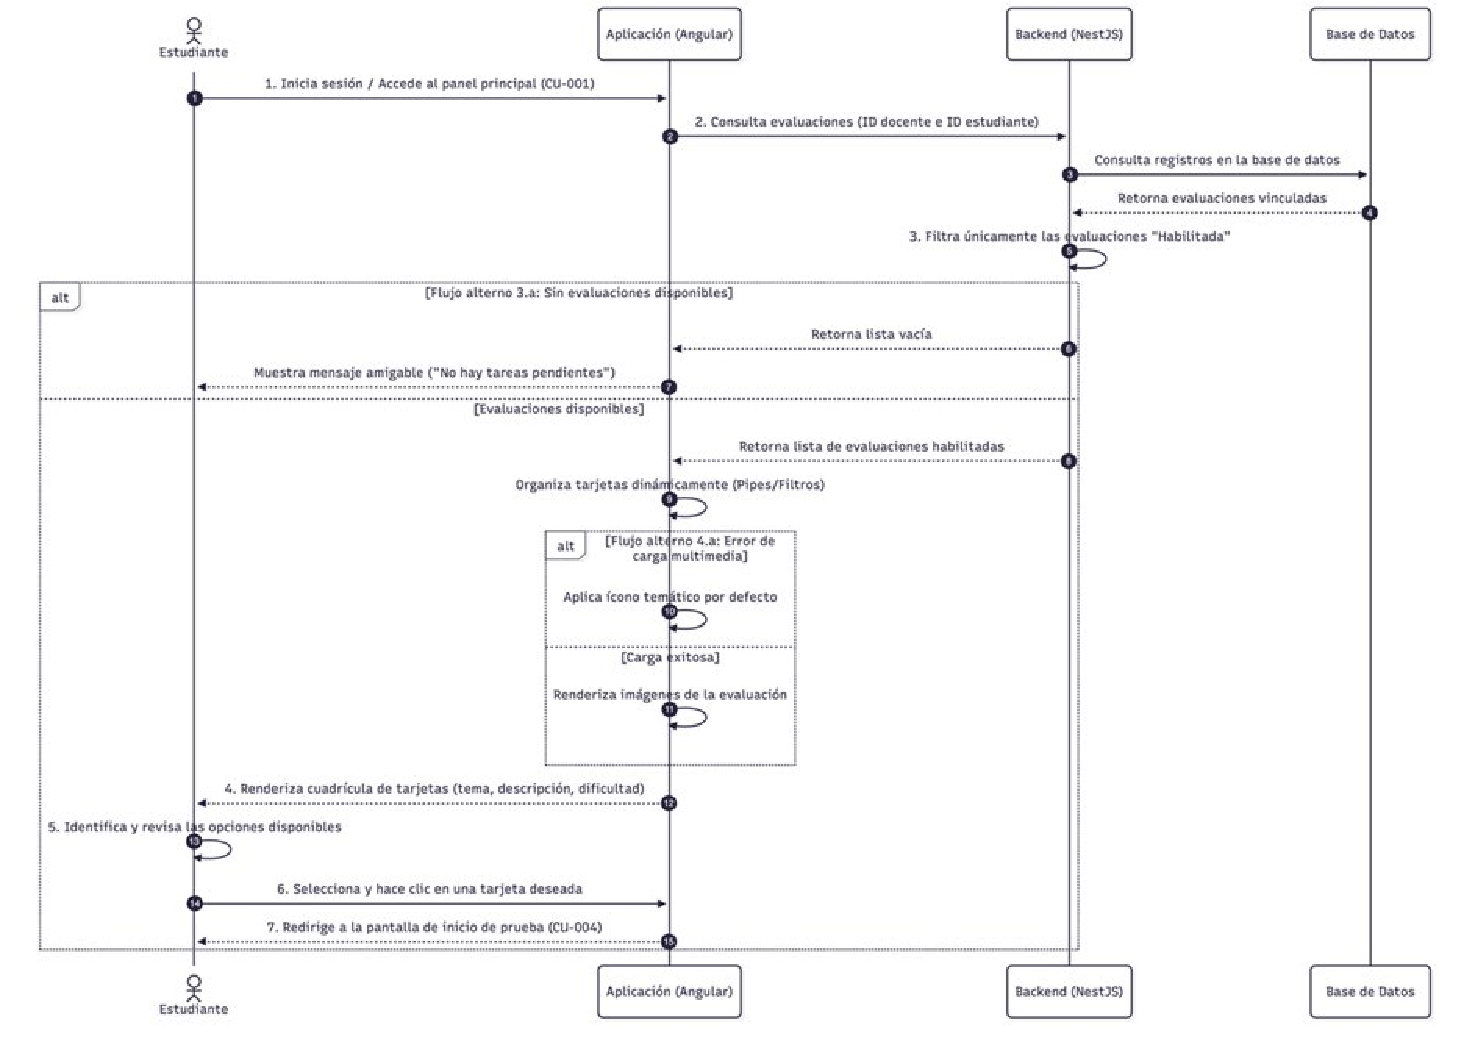
\includegraphics[width=0.92\textwidth,height=10cm,keepaspectratio]{figuras/seq_ver_eval.pdf}}\\\hline
\rowcolor{tabhead2}\multicolumn{4}{|c|}{\textbf{Interfaz de usuario}}\\\hline
\multicolumn{4}{|c|}{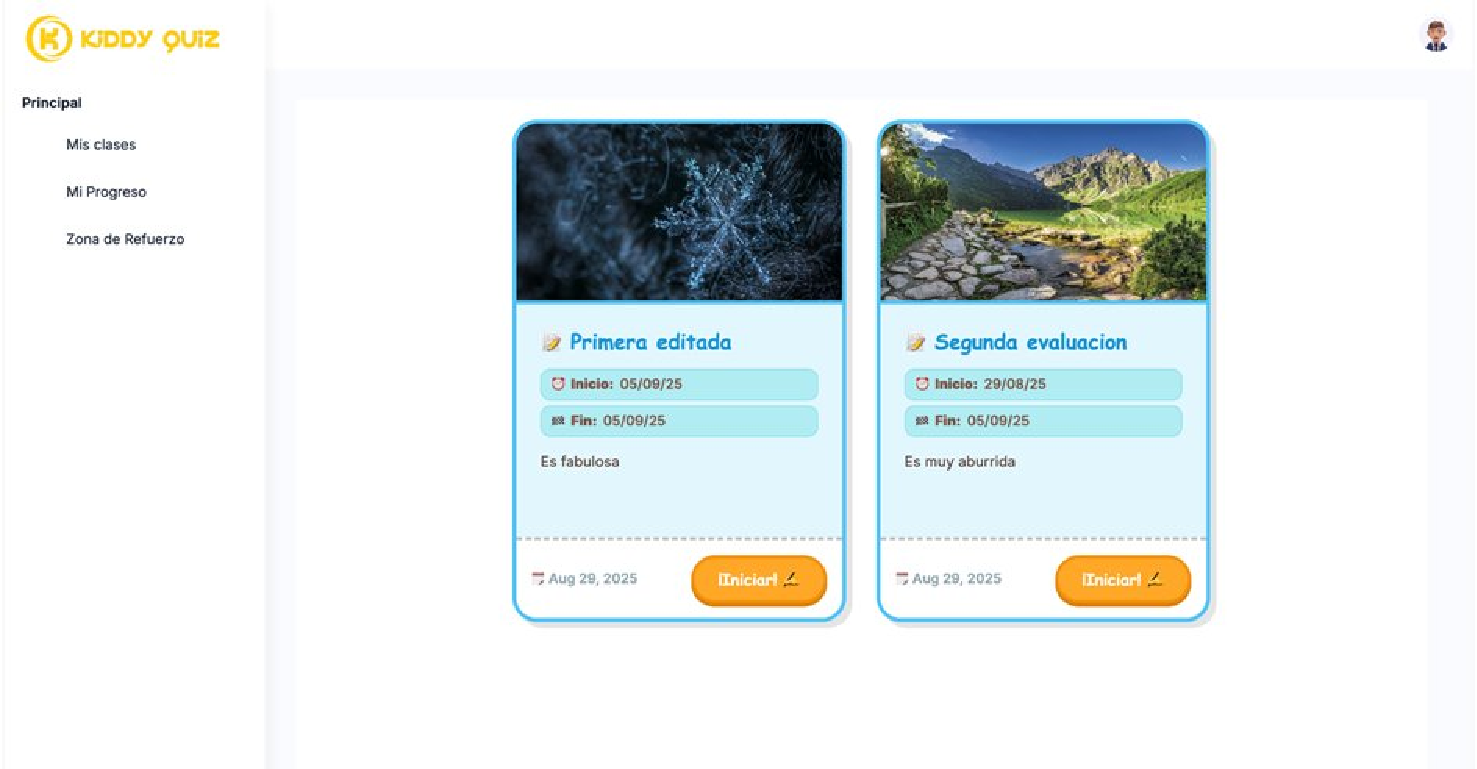
\includegraphics[width=0.92\textwidth,height=8cm,keepaspectratio]{figuras/ui_evaluaciones_estudiante.pdf}}\\\hline
Comentarios: & \multicolumn{3}{X|}{Las tarjetas deben cumplir con altos estándares de contraste y tamaño de fuente (WCAG 2.1) para asegurar la accesibilidad visual. En el \textit{frontend} con Angular, se utiliza una tubería (\textit{pipe}) o filtro para organizar dinámicamente las tarjetas por fecha o dificultad, mejorando la experiencia del niño.}\\\hline
\end{tabularx}
\end{footnotesize}
\fuenteautor
\end{table}

\begin{table}[H]
\centering
\caption{Caso de uso ``Resolver evaluación''.}
\label{tab:cu_resolver}
\begin{footnotesize}
\renewcommand{\arraystretch}{1.25}
\begin{tabularx}{\textwidth}{|>{\bfseries}L{2.6cm}|X|>{\bfseries}L{2.4cm}|X|}
\hline
\rowcolor{tabhead}\multicolumn{4}{|c|}{\tabhead{Caso de uso ``Resolver evaluación''}}\\\hline
Código: & CU-004 & Actores: & Estudiante\\\hline
Objetivo: & \multicolumn{3}{X|}{Proporcionar un entorno interactivo y amigable para que el estudiante responda las preguntas de una evaluación de forma secuencial.}\\\hline
Resumen: & \multicolumn{3}{X|}{El estudiante accede a la prueba, lee las instrucciones y responde los ítems uno a uno. El sistema permite navegación asistida, control por voz opcional y guarda el progreso automáticamente.}\\\hline
Tipo: & \multicolumn{3}{X|}{Principal}\\\hline
Dependencias: & \multicolumn{3}{X|}{\textbf{Invoca a:} CU-005 (Presentación de resultados al finalizar la evaluación). \par \textbf{Depende de:} Motor de evaluación, Base de datos de preguntas y respuestas.}\\\hline
Precondición: & \multicolumn{3}{X|}{El estudiante debe haber seleccionado una evaluación válida y habilitada desde su panel de inicio (CU-003).}\\\hline
Postcondición: & \multicolumn{3}{X|}{El sistema captura todas las respuestas y las envía al \textit{backend} para su cálculo y registro definitivo en la base de datos de desempeño.}\\\hline
[Importancia]: & \multicolumn{3}{X|}{Muy alta -- Es el núcleo funcional para los estudiantes.}\\\hline
\rowcolor{tabhead2}\multicolumn{4}{|c|}{\textbf{Flujo normal de eventos}}\\\hline
\rowcolor{tabhead2}\multicolumn{2}{|>{\columncolor{tabhead2}}c|}{\textbf{Acción del actor}} & \multicolumn{2}{>{\columncolor{tabhead2}}c|}{\textbf{Respuesta del sistema}}\\\hline
\multicolumn{2}{|X|}{1.~El estudiante selecciona una tarjeta de evaluación (CU-003).} & \multicolumn{2}{X|}{}\\\hline
\multicolumn{2}{|X|}{} & \multicolumn{2}{X|}{2.~La aplicación muestra una pantalla de ``Pre-evaluación'' con instrucciones claras.}\\\hline
\multicolumn{2}{|X|}{3.~El estudiante hace clic en el botón ``Comenzar''.} & \multicolumn{2}{X|}{}\\\hline
\multicolumn{2}{|X|}{} & \multicolumn{2}{X|}{4.~El sistema presenta la primera pregunta con sus respectivas opciones de respuesta.}\\\hline
\multicolumn{2}{|X|}{5.~(Opcional) El estudiante activa el control por voz para escuchar el enunciado.} & \multicolumn{2}{X|}{6.~El sistema sintetiza el texto y reproduce el audio del ítem actual.}\\\hline
\multicolumn{2}{|X|}{7.~El estudiante selecciona una respuesta y hace clic en el botón ``Siguiente''.} & \multicolumn{2}{X|}{}\\\hline
\multicolumn{2}{|X|}{} & \multicolumn{2}{X|}{8.~El sistema guarda la respuesta temporalmente y carga el siguiente ítem secuencialmente.}\\\hline
\multicolumn{2}{|X|}{9.~El estudiante repite los pasos 7 y 8 hasta completar todos los ítems de la prueba.} & \multicolumn{2}{X|}{}\\\hline
\multicolumn{2}{|X|}{10.~Al finalizar la última pregunta, el estudiante hace clic en el botón ``Finalizar''.} & \multicolumn{2}{X|}{}\\\hline
\multicolumn{2}{|X|}{} & \multicolumn{2}{X|}{11.~El sistema procesa los datos y redirige a la pantalla de resultados (CU-005).}\\\hline
\rowcolor{tabhead2}\multicolumn{4}{|c|}{\textbf{Flujo alterno}}\\\hline
\multicolumn{4}{|X|}{\textbf{4.a.\ Evaluación con tiempo límite:} el sistema inicia un contador regresivo; si el tiempo se agota, se guarda lo avanzado y se finaliza la prueba automáticamente. \par \textbf{6.a.\ Error de reproducción de voz:} si el navegador no soporta el audio, el sistema muestra una alerta sugiriendo continuar con la lectura visual. \par \textbf{8.a.\ Desconexión de internet:} el sistema notifica la pérdida de conexión y mantiene las respuestas en caché local hasta que se restablezca el servicio.}\\\hline
\rowcolor{tabhead2}\multicolumn{4}{|c|}{\textbf{Diagrama de secuencia}}\\\hline
\multicolumn{4}{|c|}{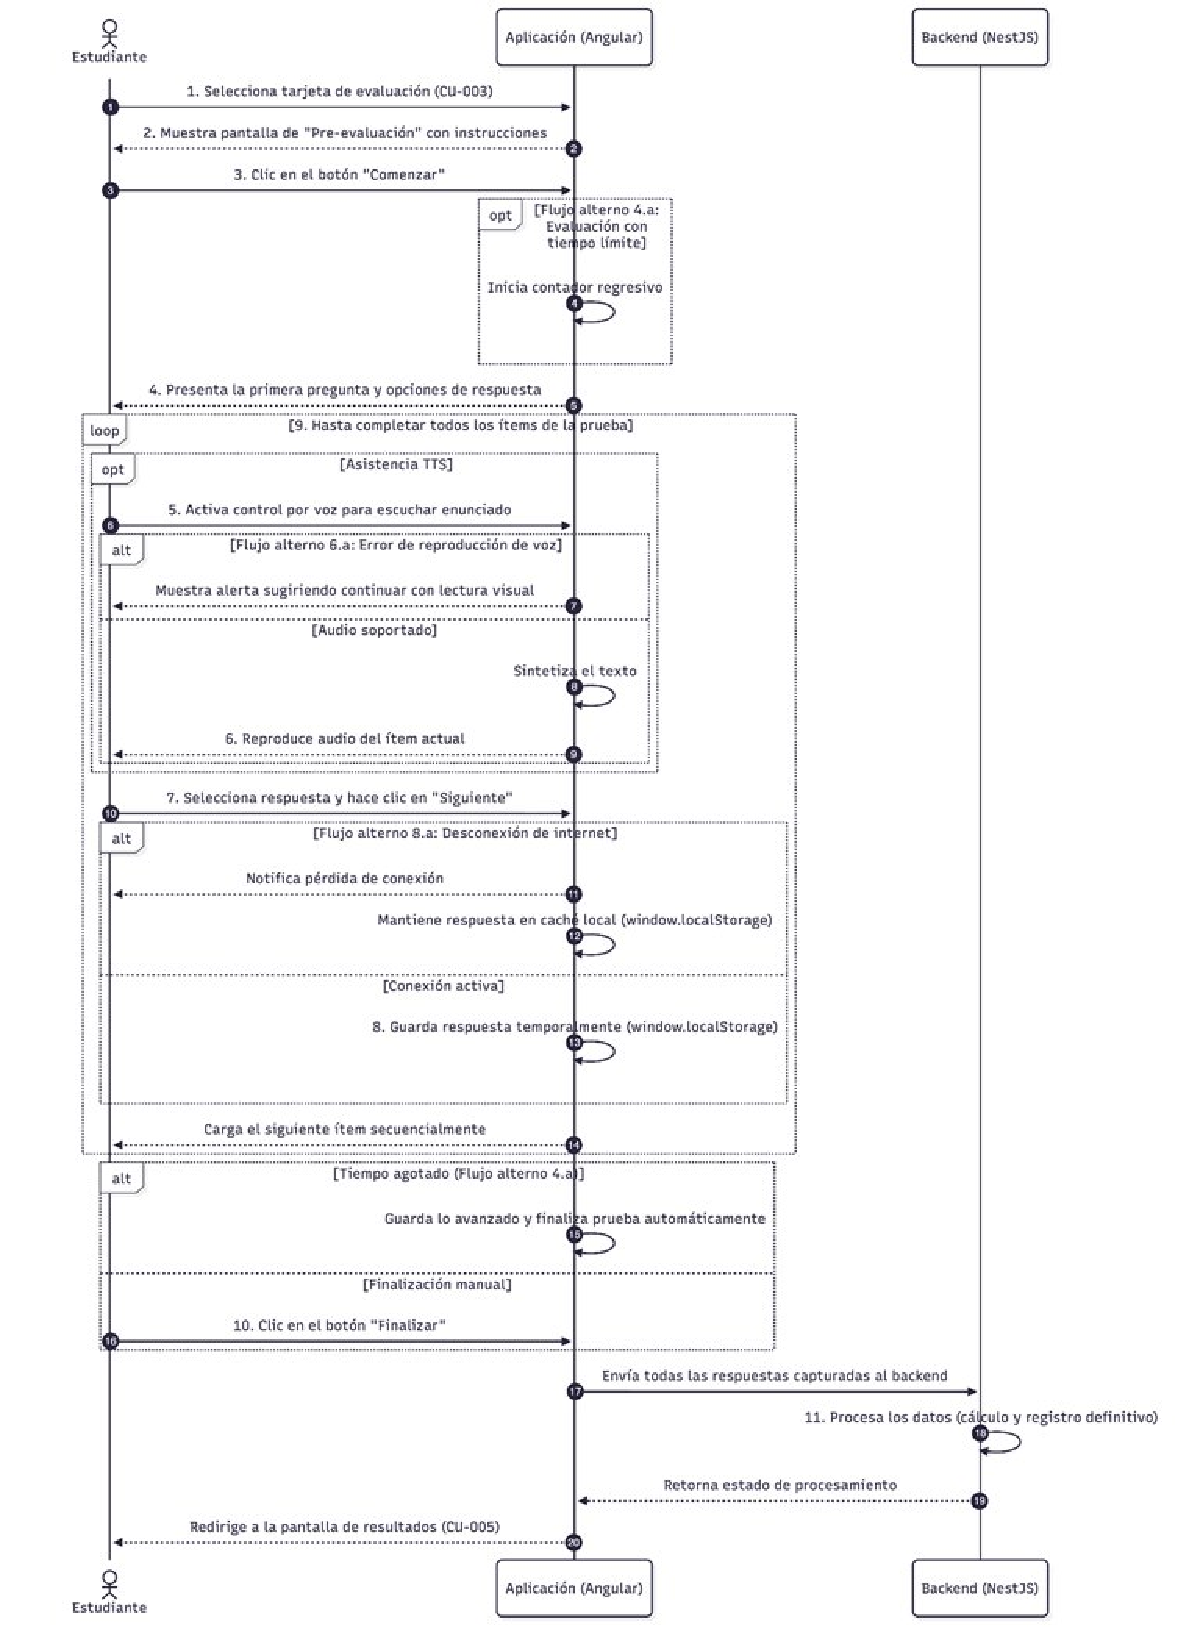
\includegraphics[width=0.92\textwidth,height=10cm,keepaspectratio]{figuras/seq_resolver_eval.pdf}}\\\hline
\rowcolor{tabhead2}\multicolumn{4}{|c|}{\textbf{Interfaz de usuario}}\\\hline
\multicolumn{4}{|c|}{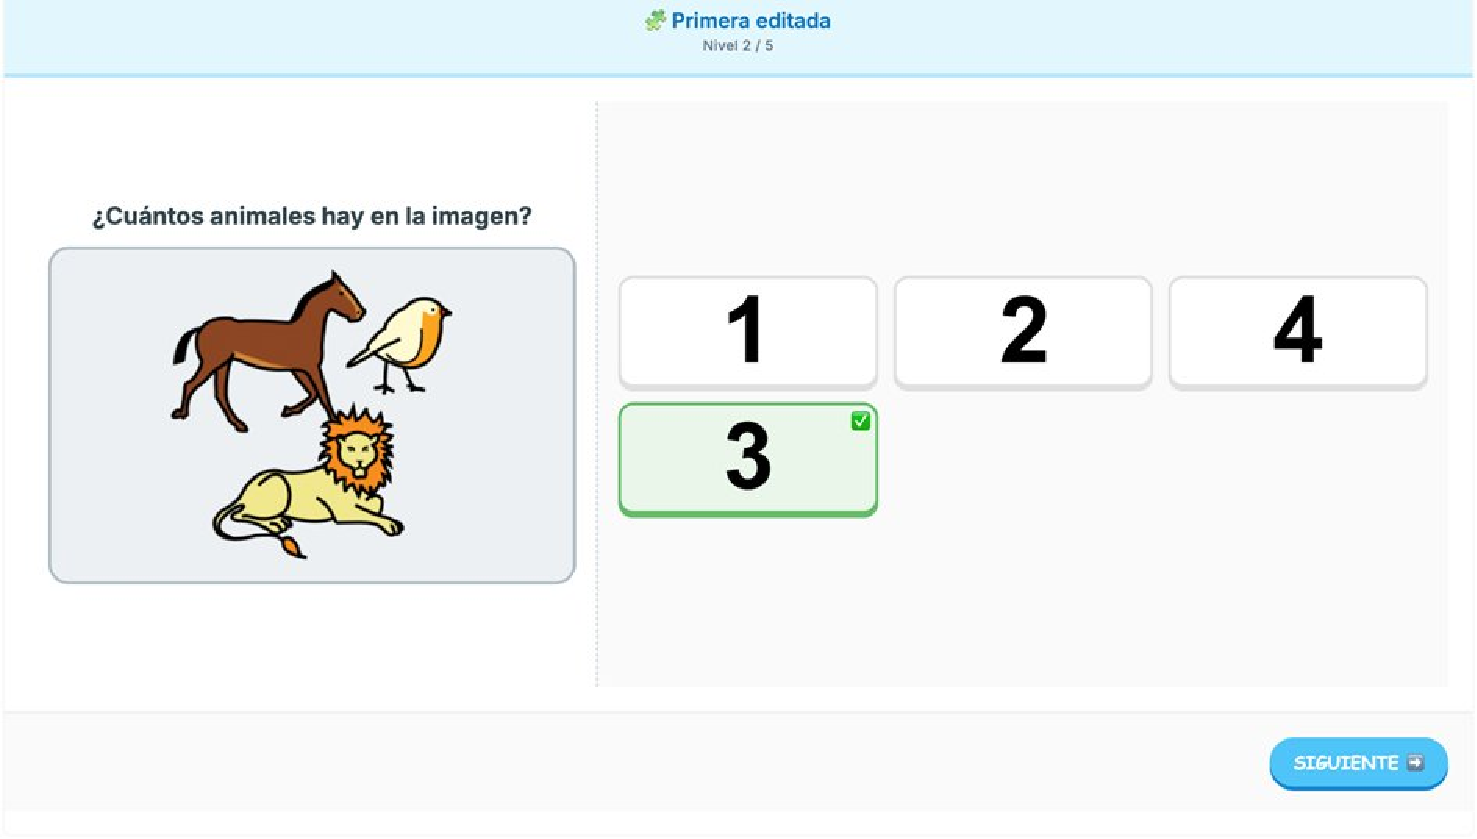
\includegraphics[width=0.92\textwidth,height=8cm,keepaspectratio]{figuras/ui_resolver_eval_pictograma.pdf}}\\\hline
Comentarios: & \multicolumn{3}{X|}{La interfaz debe ser 100\,\% responsiva y optimizada para dispositivos táctiles (\textit{tablets}), facilitando la interacción de niños de primaria. El uso de \texttt{window.localStorage} en Angular asegura que el progreso no se pierda ante cierres accidentales de la pestaña del navegador.}\\\hline
\end{tabularx}
\end{footnotesize}
\fuenteautor
\end{table}

\begin{table}[H]
\centering
\caption{Caso de uso ``Ver retroalimentación''.}
\label{tab:cu_retro}
\begin{footnotesize}
\renewcommand{\arraystretch}{1.25}
\begin{tabularx}{\textwidth}{|>{\bfseries}L{2.6cm}|X|>{\bfseries}L{2.4cm}|X|}
\hline
\rowcolor{tabhead}\multicolumn{4}{|c|}{\tabhead{Caso de uso ``Ver retroalimentación''}}\\\hline
Código: & CU-005 & Actores: & Estudiante\\\hline
Objetivo: & \multicolumn{3}{X|}{Proporcionar al estudiante una visualización clara y motivadora de su desempeño académico inmediatamente después de completar una prueba.}\\\hline
Resumen: & \multicolumn{3}{X|}{El sistema calcula la calificación, el tiempo empleado y genera una retroalimentación gráfica y motivacional para informar al estudiante sobre sus logros.}\\\hline
Tipo: & \multicolumn{3}{X|}{Principal}\\\hline
Dependencias: & \multicolumn{3}{X|}{\textbf{Invoca a:} retorno a la pantalla principal (CU-003). \par \textbf{Depende de:} Módulo de corrección automática, Sistema gráfico de resultados y Base de datos de desempeño.}\\\hline
Precondición: & \multicolumn{3}{X|}{El estudiante debe haber finalizado y enviado satisfactoriamente las respuestas de su evaluación (CU-004). El \textit{backend} debe haber procesado y calculado la calificación final.}\\\hline
Postcondición: & \multicolumn{3}{X|}{El estudiante visualiza su rendimiento y el estado de la evaluación cambia a ``Completada'' en la base de datos.}\\\hline
[Importancia]: & \multicolumn{3}{X|}{Alta -- Aporta retroalimentación y cierre al proceso de aprendizaje.}\\\hline
\rowcolor{tabhead2}\multicolumn{4}{|c|}{\textbf{Flujo normal de eventos}}\\\hline
\rowcolor{tabhead2}\multicolumn{2}{|>{\columncolor{tabhead2}}c|}{\textbf{Acción del actor}} & \multicolumn{2}{>{\columncolor{tabhead2}}c|}{\textbf{Respuesta del sistema}}\\\hline
\multicolumn{2}{|X|}{1.~El estudiante hace clic en el botón ``Finalizar'' de la evaluación (CU-004).} & \multicolumn{2}{X|}{}\\\hline
\multicolumn{2}{|X|}{} & \multicolumn{2}{X|}{2.~El sistema recibe las respuestas y ejecuta el algoritmo de calificación automática.}\\\hline
\multicolumn{2}{|X|}{} & \multicolumn{2}{X|}{3.~El sistema calcula el tiempo total empleado durante la sesión de prueba.}\\\hline
\multicolumn{2}{|X|}{} & \multicolumn{2}{X|}{4.~La aplicación renderiza una pantalla de resultados con el puntaje numérico obtenido.}\\\hline
\multicolumn{2}{|X|}{} & \multicolumn{2}{X|}{5.~El sistema genera y muestra un gráfico de desempeño (barras o pastel) con colores amigables.}\\\hline
\multicolumn{2}{|X|}{} & \multicolumn{2}{X|}{6.~El sistema muestra una imagen de \textit{feedback} motivacional (medalla o estrella) basada en el rango de nota.}\\\hline
\multicolumn{2}{|X|}{7.~(Opcional) El estudiante selecciona ``Revisar respuestas'' si el docente habilitó la opción.} & \multicolumn{2}{X|}{8.~El sistema despliega el detalle de aciertos y errores cometidos.}\\\hline
\multicolumn{2}{|X|}{9.~El estudiante hace clic en ``Volver al inicio''.} & \multicolumn{2}{X|}{}\\\hline
\multicolumn{2}{|X|}{} & \multicolumn{2}{X|}{10.~La aplicación redirige al estudiante a su panel principal de evaluaciones (CU-003).}\\\hline
\rowcolor{tabhead2}\multicolumn{4}{|c|}{\textbf{Flujo alterno}}\\\hline
\multicolumn{4}{|X|}{\textbf{2.a.\ Error en el procesamiento:} si el cálculo de la nota falla, el sistema muestra un mensaje de error y guarda las respuestas para un reintento automático de calificación posterior. \par \textbf{8.a.\ Revisión deshabilitada:} si el docente no permitió la revisión, el botón correspondiente no aparecerá en la interfaz de resultados.}\\\hline
\rowcolor{tabhead2}\multicolumn{4}{|c|}{\textbf{Diagrama de secuencia}}\\\hline
\multicolumn{4}{|c|}{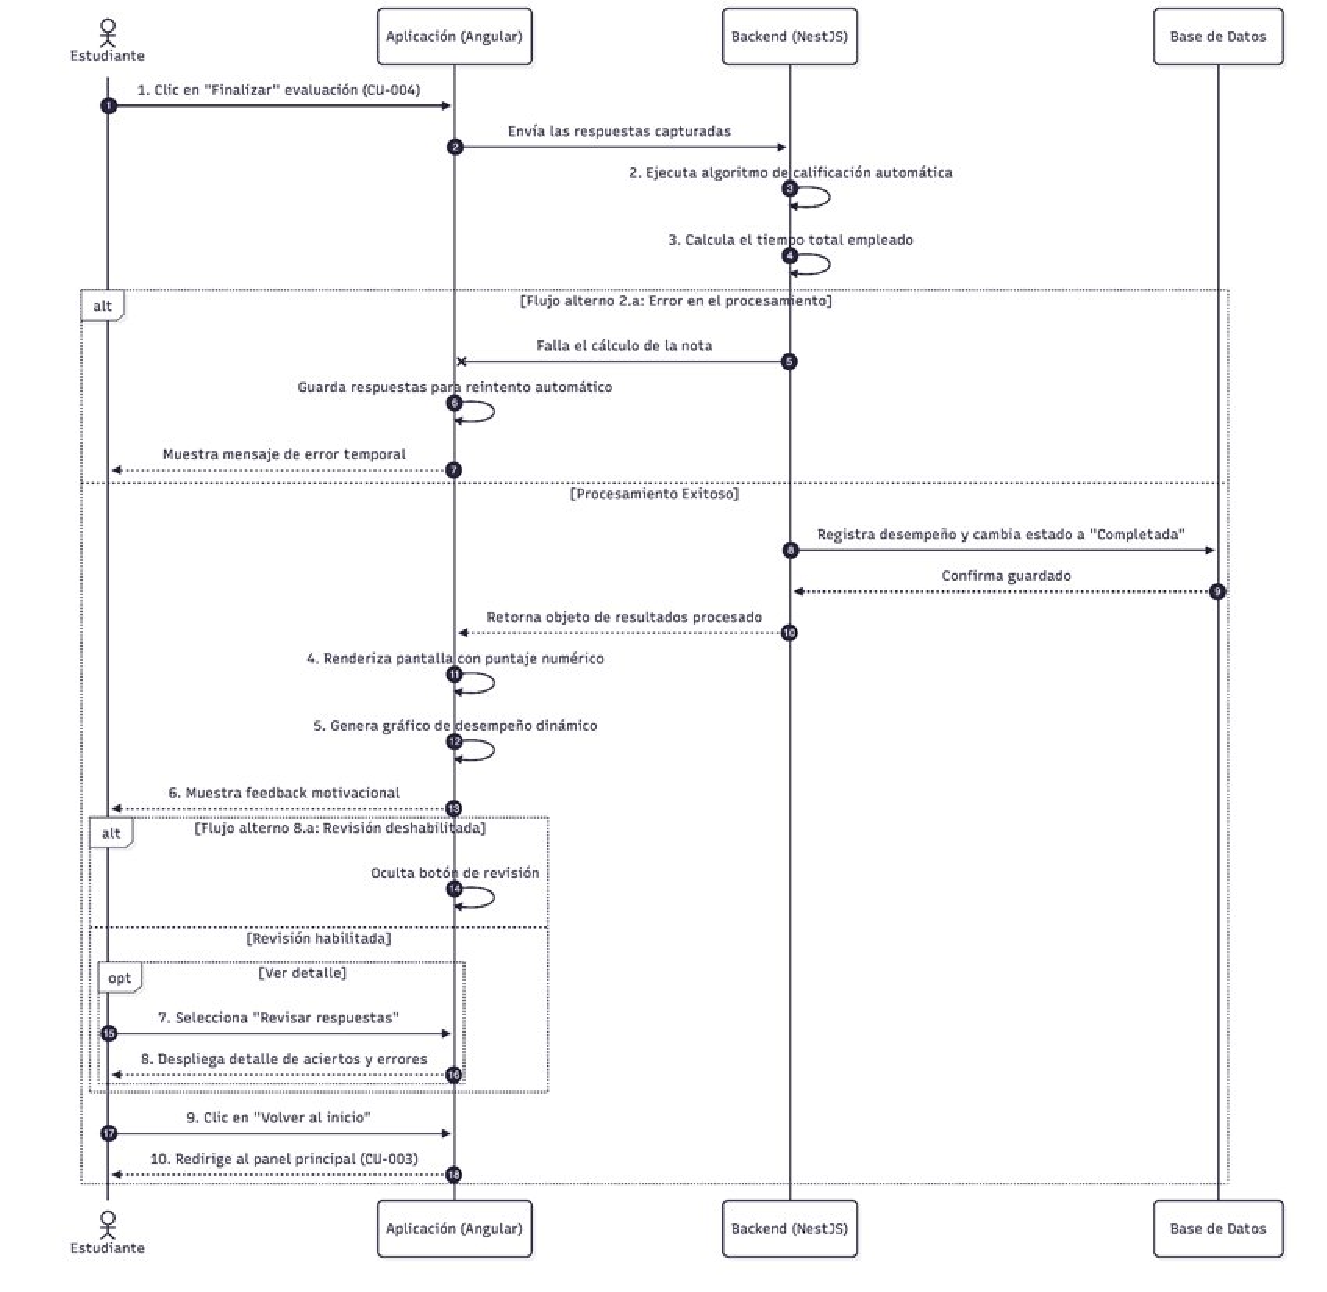
\includegraphics[width=0.92\textwidth,height=10cm,keepaspectratio]{figuras/seq_ver_retroalimentacion.pdf}}\\\hline
\rowcolor{tabhead2}\multicolumn{4}{|c|}{\textbf{Interfaz de usuario}}\\\hline
\multicolumn{4}{|c|}{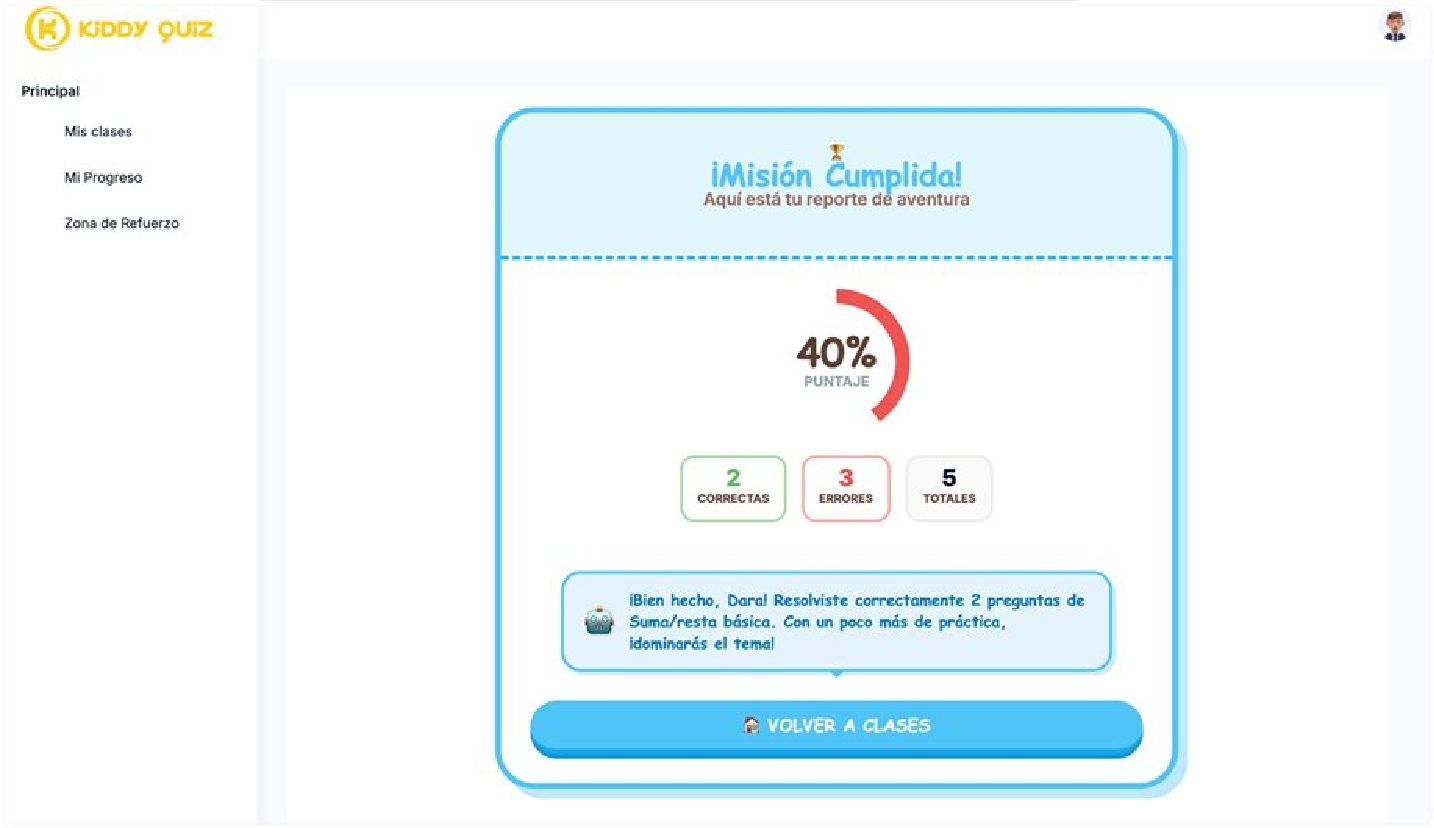
\includegraphics[width=0.92\textwidth,height=8cm,keepaspectratio]{figuras/ui_retroalimentacion.pdf}}\\\hline
Comentarios: & \multicolumn{3}{X|}{Los mensajes motivacionales deben estar adaptados a niños de primaria (ej. ``¡Excelente!'', ``¡Sigue así!''). Técnicamente, Angular recibe el objeto de resultados procesado por NestJS y utiliza librerías de gráficos para pintar la información de forma dinámica y responsiva.}\\\hline
\end{tabularx}
\end{footnotesize}
\fuenteautor
\end{table}

\begin{table}[H]
\centering
\caption{Caso de uso ``Gestionar panel docente''.}
\label{tab:cu_panel}
\begin{footnotesize}
\renewcommand{\arraystretch}{1.25}
\begin{tabularx}{\textwidth}{|>{\bfseries}L{2.6cm}|X|>{\bfseries}L{2.4cm}|X|}
\hline
\rowcolor{tabhead}\multicolumn{4}{|c|}{\tabhead{Caso de uso ``Gestionar panel docente''}}\\\hline
Código: & CU-006 & Actores: & Docente\\\hline
Objetivo: & \multicolumn{3}{X|}{Visualizar todas las evaluaciones que el docente ha creado organizadas en formato de tarjetas informativas desde su pantalla principal.}\\\hline
Resumen: & \multicolumn{3}{X|}{El docente accede a su panel principal donde el sistema filtra y muestra exclusivamente sus evaluaciones creadas, permitiéndole conocer su estado de visibilidad y acceder a su edición.}\\\hline
Tipo: & \multicolumn{3}{X|}{Principal}\\\hline
Dependencias: & \multicolumn{3}{X|}{\textbf{Invoca a:} CU-008 (Creación de evaluaciones) y CU-007 (Habilitación y deshabilitación). \par \textbf{Depende de:} Base de datos de evaluaciones, Autenticación y perfil docente.}\\\hline
Precondición: & \multicolumn{3}{X|}{El docente debe haber iniciado sesión en el sistema y tener un \textit{token} de autenticación válido.}\\\hline
Postcondición: & \multicolumn{3}{X|}{El sistema despliega la lista de tarjetas correspondientes a las pruebas creadas por el docente, habilitando el acceso rápido a la edición de cada una.}\\\hline
[Importancia]: & \multicolumn{3}{X|}{Alta -- Facilita la gestión directa del contenido por parte del docente.}\\\hline
\rowcolor{tabhead2}\multicolumn{4}{|c|}{\textbf{Flujo normal de eventos}}\\\hline
\rowcolor{tabhead2}\multicolumn{2}{|>{\columncolor{tabhead2}}c|}{\textbf{Acción del actor}} & \multicolumn{2}{>{\columncolor{tabhead2}}c|}{\textbf{Respuesta del sistema}}\\\hline
\multicolumn{2}{|X|}{1.~El docente inicia sesión exitosamente en la plataforma (CU-001).} & \multicolumn{2}{X|}{}\\\hline
\multicolumn{2}{|X|}{} & \multicolumn{2}{X|}{2.~El sistema identifica el ID del docente autenticado en la base de datos.}\\\hline
\multicolumn{2}{|X|}{} & \multicolumn{2}{X|}{3.~El sistema filtra exclusivamente las evaluaciones asociadas a dicho ID.}\\\hline
\multicolumn{2}{|X|}{} & \multicolumn{2}{X|}{4.~La aplicación renderiza en el panel principal una cuadrícula con tarjetas informativas.}\\\hline
\multicolumn{2}{|X|}{5.~El docente revisa el nombre, descripción, nivel de dificultad y estado (habilitada/deshabilitada) de sus pruebas.} & \multicolumn{2}{X|}{}\\\hline
\multicolumn{2}{|X|}{6.~El docente selecciona el ícono de ``acceso rápido'' en una tarjeta específica.} & \multicolumn{2}{X|}{}\\\hline
\multicolumn{2}{|X|}{} & \multicolumn{2}{X|}{7.~La aplicación redirige al docente a la interfaz de edición de esa evaluación.}\\\hline
\rowcolor{tabhead2}\multicolumn{4}{|c|}{\textbf{Flujo alterno}}\\\hline
\multicolumn{4}{|X|}{\textbf{3.a.\ Docente sin evaluaciones:} si el docente no ha creado contenido aún, el sistema muestra un mensaje indicando que la lista está vacía y ofrece un botón destacado para ``Crear nueva evaluación''. \par \textbf{4.a.\ Error de carga de datos:} si el servidor no responde, la interfaz muestra una alerta de error de conexión y permite reintentar la carga del panel.}\\\hline
\rowcolor{tabhead2}\multicolumn{4}{|c|}{\textbf{Diagrama de secuencia}}\\\hline
\multicolumn{4}{|c|}{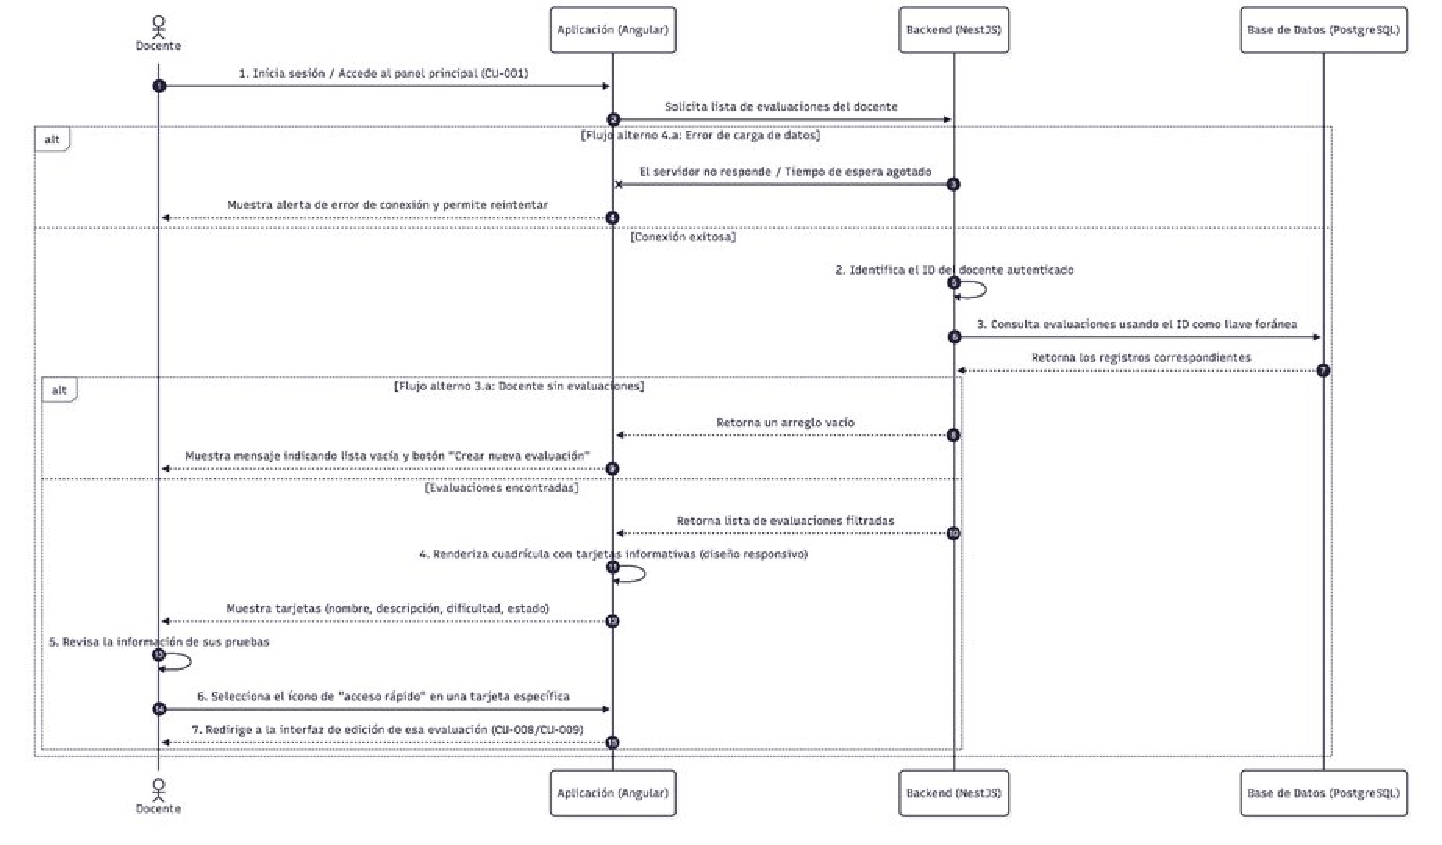
\includegraphics[width=0.92\textwidth,height=10cm,keepaspectratio]{figuras/seq_panel_docente.pdf}}\\\hline
\rowcolor{tabhead2}\multicolumn{4}{|c|}{\textbf{Interfaz de usuario}}\\\hline
\multicolumn{4}{|c|}{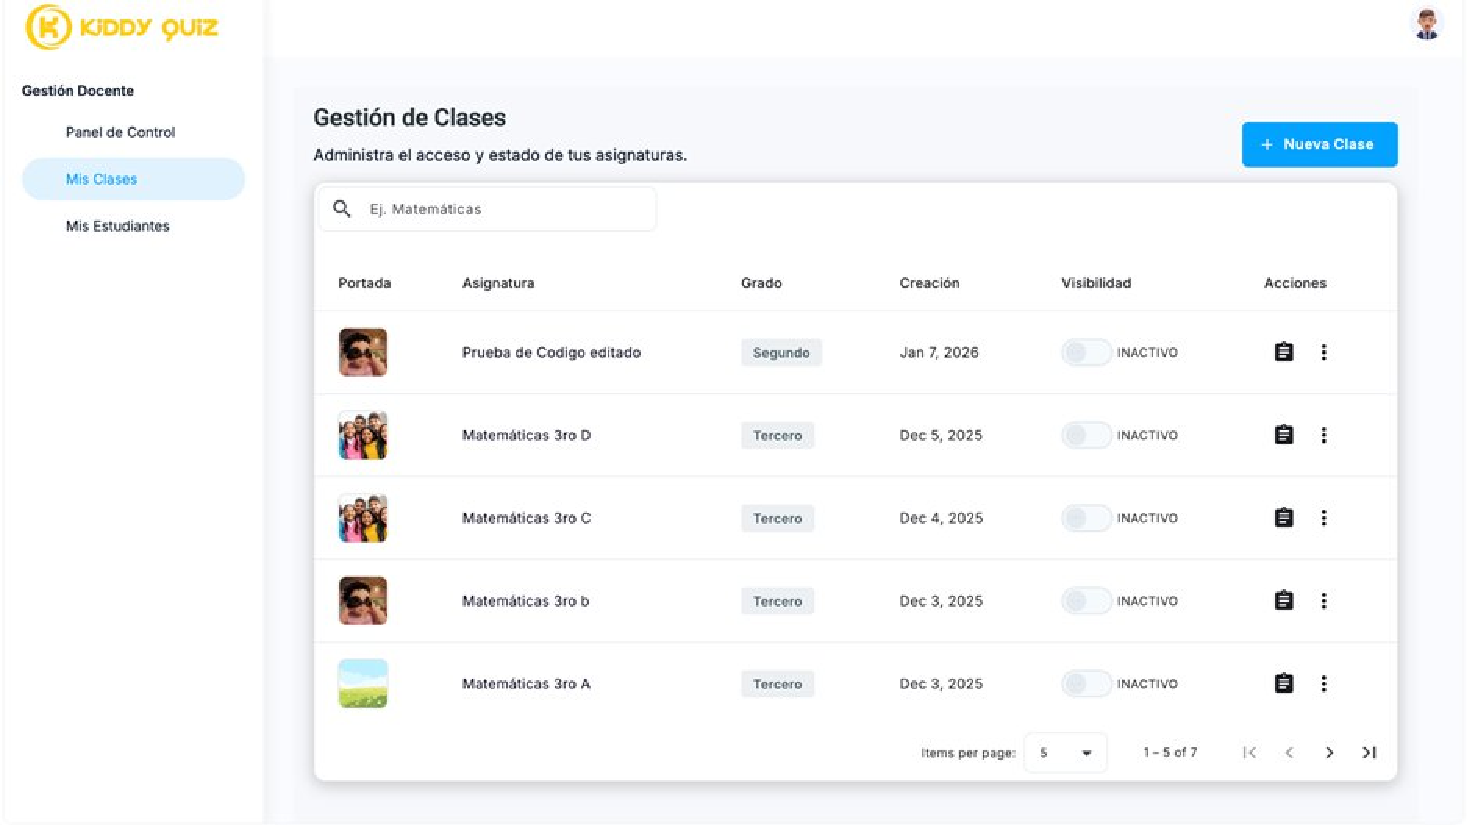
\includegraphics[width=0.92\textwidth,height=8cm,keepaspectratio]{figuras/ui_panel_docente_clases.pdf}}\\\hline
Comentarios: & \multicolumn{3}{X|}{El diseño debe ser totalmente responsivo, garantizando que el docente pueda gestionar sus evaluaciones desde computadoras o dispositivos móviles. En la base de datos PostgreSQL se utiliza el ID del docente como llave foránea para asegurar que un profesor no pueda visualizar ni editar las pruebas de otro colega.}\\\hline
\end{tabularx}
\end{footnotesize}
\fuenteautor
\end{table}

\begin{table}[H]
\centering
\caption{Caso de uso ``Crear examen''.}
\label{tab:cu_crear_examen}
\begin{footnotesize}
\renewcommand{\arraystretch}{1.25}
\begin{tabularx}{\textwidth}{|>{\bfseries}L{2.6cm}|X|>{\bfseries}L{2.4cm}|X|}
\hline
\rowcolor{tabhead}\multicolumn{4}{|c|}{\tabhead{Caso de uso ``Crear examen''}}\\\hline
Código: & CU-008 & Actores: & Docente\\\hline
Objetivo: & \multicolumn{3}{X|}{Permitir al docente definir la estructura base de una nueva evaluación (tema, dificultad, descripción y duración) antes de agregar las preguntas.}\\\hline
Resumen: & \multicolumn{3}{X|}{El docente ingresa los datos generales de la prueba en un formulario; el sistema valida la información y crea el registro de la evaluación en la base de datos en estado inactivo o borrador.}\\\hline
Tipo: & \multicolumn{3}{X|}{Principal}\\\hline
Dependencias: & \multicolumn{3}{X|}{\textbf{Invoca a:} CU-009 (Gestión de preguntas por evaluación). \par \textbf{Depende de:} Interfaz de gestión docente y Base de datos de evaluaciones.}\\\hline
Precondición: & \multicolumn{3}{X|}{El docente debe haber iniciado sesión exitosamente, contar con los permisos adecuados y encontrarse en su panel de gestión.}\\\hline
Postcondición: & \multicolumn{3}{X|}{La nueva evaluación queda registrada en la base de datos vinculada al docente, habilitando la interfaz para comenzar a agregarle preguntas.}\\\hline
[Importancia]: & \multicolumn{3}{X|}{Muy alta -- Es la funcionalidad base del sistema de evaluación.}\\\hline
\rowcolor{tabhead2}\multicolumn{4}{|c|}{\textbf{Flujo normal de eventos}}\\\hline
\rowcolor{tabhead2}\multicolumn{2}{|>{\columncolor{tabhead2}}c|}{\textbf{Acción del actor}} & \multicolumn{2}{>{\columncolor{tabhead2}}c|}{\textbf{Respuesta del sistema}}\\\hline
\multicolumn{2}{|X|}{1.~El docente selecciona la opción ``Crear nueva evaluación''.} & \multicolumn{2}{X|}{}\\\hline
\multicolumn{2}{|X|}{} & \multicolumn{2}{X|}{2.~El sistema muestra el formulario vacío de creación de evaluación.}\\\hline
\multicolumn{2}{|X|}{3.~El docente completa los campos obligatorios: título/tema, nivel de dificultad, descripción y duración (minutos).} & \multicolumn{2}{X|}{}\\\hline
\multicolumn{2}{|X|}{4.~El docente hace clic en el botón ``Crear evaluación''.} & \multicolumn{2}{X|}{}\\\hline
\multicolumn{2}{|X|}{} & \multicolumn{2}{X|}{5.~El sistema valida que los campos requeridos no estén vacíos y que la duración sea mayor a cero.}\\\hline
\multicolumn{2}{|X|}{} & \multicolumn{2}{X|}{6.~El sistema registra la nueva evaluación en la base de datos (PostgreSQL).}\\\hline
\multicolumn{2}{|X|}{} & \multicolumn{2}{X|}{7.~La aplicación redirige al docente a la interfaz de gestión de preguntas (CU-009).}\\\hline
\rowcolor{tabhead2}\multicolumn{4}{|c|}{\textbf{Flujo alterno}}\\\hline
\multicolumn{4}{|X|}{\textbf{5.a.} Si el docente deja campos obligatorios vacíos, el sistema resalta los errores en rojo y detiene el proceso de guardado. \par \textbf{5.b.} Si se ingresa una duración negativa o cero, el sistema solicita ingresar un número válido antes de continuar.}\\\hline
\rowcolor{tabhead2}\multicolumn{4}{|c|}{\textbf{Diagrama de secuencia}}\\\hline
\multicolumn{4}{|c|}{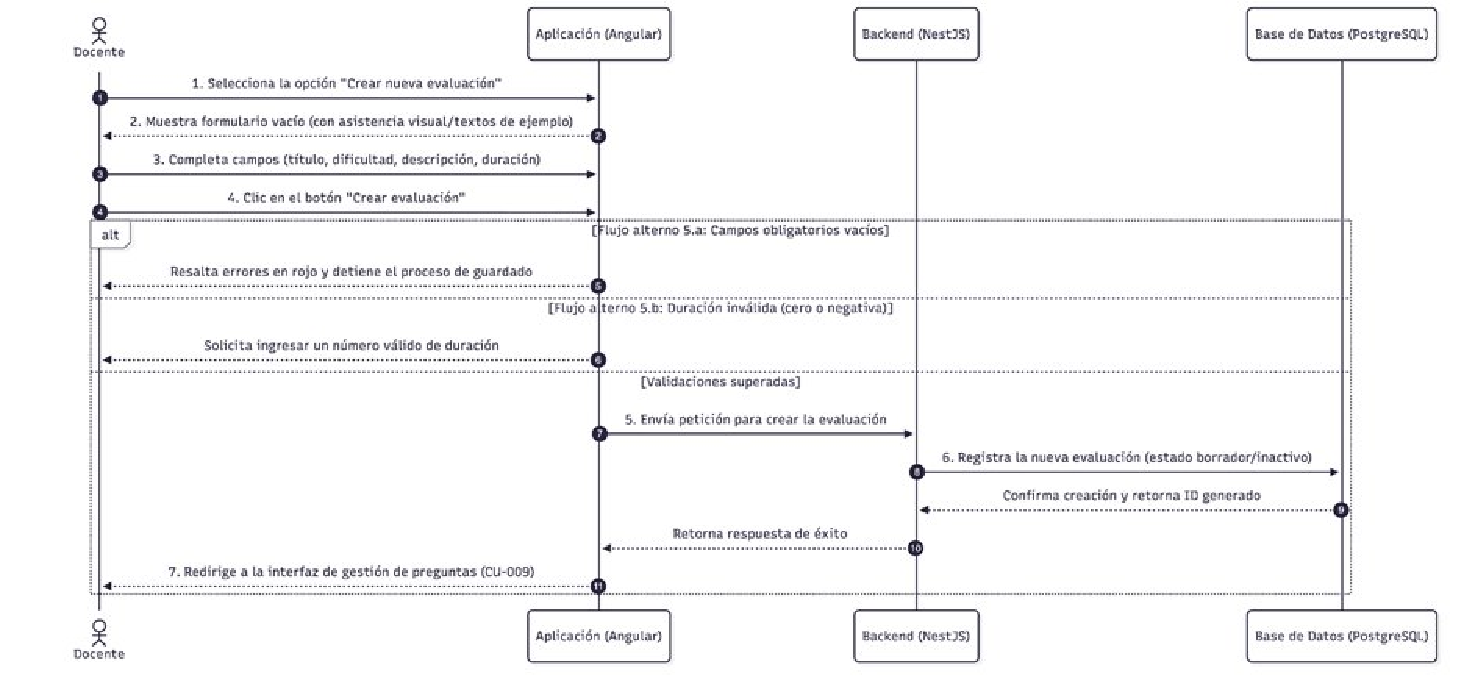
\includegraphics[width=0.92\textwidth,height=10cm,keepaspectratio]{figuras/seq_crear_examen.pdf}}\\\hline
\rowcolor{tabhead2}\multicolumn{4}{|c|}{\textbf{Interfaz de usuario}}\\\hline
\multicolumn{4}{|c|}{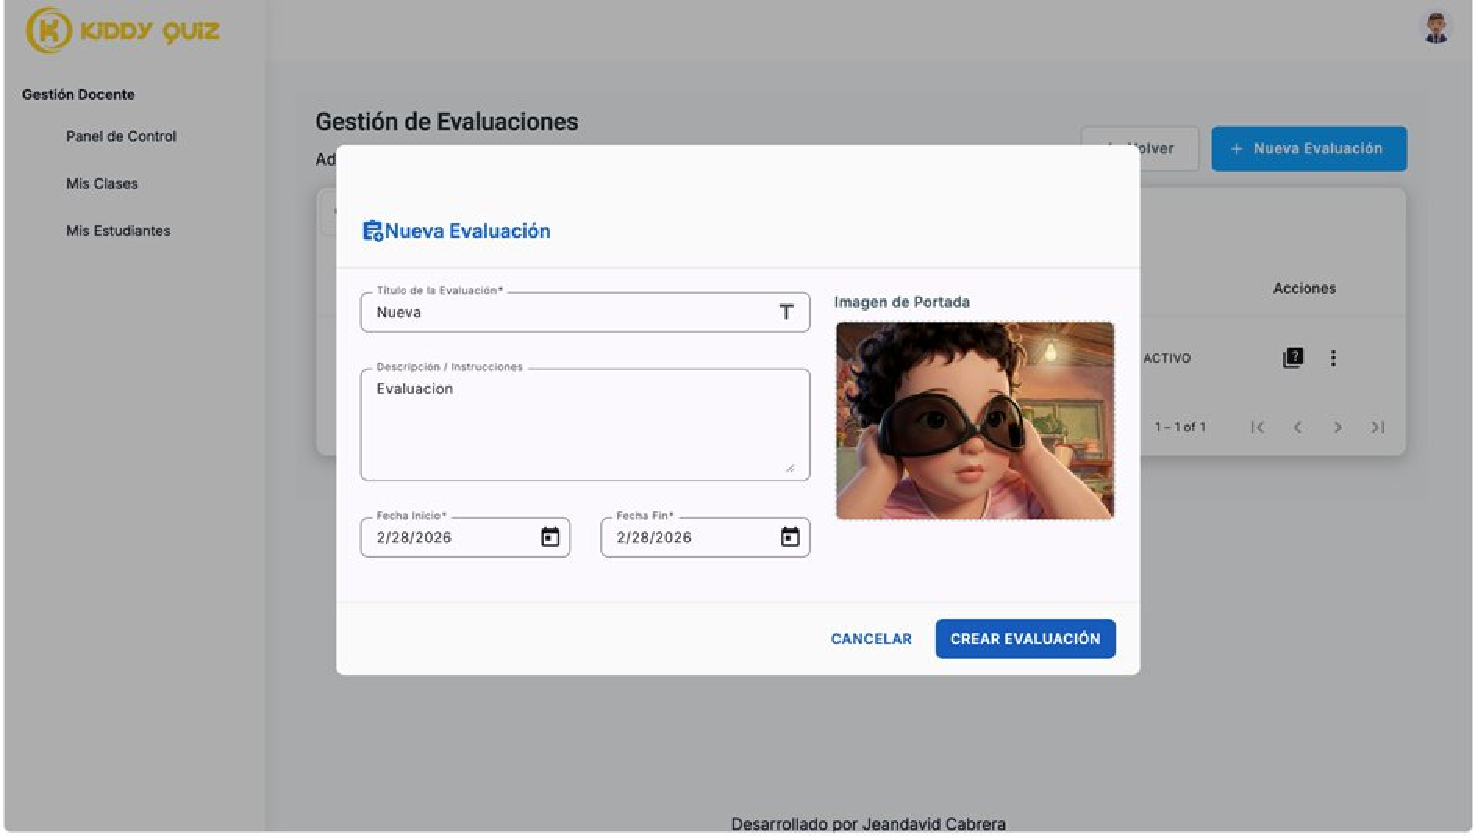
\includegraphics[width=0.92\textwidth,height=8cm,keepaspectratio]{figuras/ui_crear_examen.pdf}}\\\hline
Comentarios: & \multicolumn{3}{X|}{Se recomienda agregar asistencia visual en la interfaz (como textos de ejemplo tenues en los campos vacíos o plantillas prediseñadas) para facilitar la carga de datos al docente.}\\\hline
\end{tabularx}
\end{footnotesize}
\fuenteautor
\end{table}

\begin{table}[H]
\centering
\caption{Caso de uso ``Organizar preguntas''.}
\label{tab:cu_org_preg}
\begin{footnotesize}
\renewcommand{\arraystretch}{1.25}
\begin{tabularx}{\textwidth}{|>{\bfseries}L{2.6cm}|X|>{\bfseries}L{2.4cm}|X|}
\hline
\rowcolor{tabhead}\multicolumn{4}{|c|}{\tabhead{Caso de uso ``Organizar preguntas''}}\\\hline
Código: & CU-009 & Actores: & Docente\\\hline
Objetivo: & \multicolumn{3}{X|}{Permitir al docente gestionar la lista de preguntas asociadas a una evaluación específica mediante funciones de visualización, edición, eliminación y reordenamiento.}\\\hline
Resumen: & \multicolumn{3}{X|}{El docente accede al administrador de una prueba para ver y modificar las preguntas existentes. El sistema procesa estas acciones (CRUD y ordenamiento) y actualiza la estructura de la evaluación en la base de datos.}\\\hline
Tipo: & \multicolumn{3}{X|}{Principal}\\\hline
Dependencias: & \multicolumn{3}{X|}{\textbf{Invoca a:} CU-010 (Creación de preguntas). \par \textbf{Depende de:} Evaluación previamente creada (CU-008) y base de datos de preguntas.}\\\hline
Precondición: & \multicolumn{3}{X|}{El docente debe haber iniciado sesión y debe haber creado previamente al menos una evaluación.}\\\hline
Postcondición: & \multicolumn{3}{X|}{El sistema actualiza la estructura de la evaluación en la base de datos, reflejando cualquier modificación, eliminación o cambio de orden.}\\\hline
[Importancia]: & \multicolumn{3}{X|}{Muy alta -- Fundamental para personalizar y estructurar las evaluaciones.}\\\hline
\rowcolor{tabhead2}\multicolumn{4}{|c|}{\textbf{Flujo normal de eventos}}\\\hline
\rowcolor{tabhead2}\multicolumn{2}{|>{\columncolor{tabhead2}}c|}{\textbf{Acción del actor}} & \multicolumn{2}{>{\columncolor{tabhead2}}c|}{\textbf{Respuesta del sistema}}\\\hline
\multicolumn{2}{|X|}{1.~El docente selecciona una evaluación y da clic en ``Gestionar preguntas''.} & \multicolumn{2}{X|}{}\\\hline
\multicolumn{2}{|X|}{} & \multicolumn{2}{X|}{2.~El sistema consulta y muestra la lista editable con todas las preguntas asociadas a esa prueba.}\\\hline
\multicolumn{2}{|X|}{3.~El docente interactúa con la lista cambiando el orden de las preguntas (arrastrar y soltar).} & \multicolumn{2}{X|}{}\\\hline
\multicolumn{2}{|X|}{} & \multicolumn{2}{X|}{4.~El sistema actualiza visualmente el orden de la lista en la pantalla.}\\\hline
\multicolumn{2}{|X|}{5.~El docente da clic en el botón de guardar o confirmar cambios.} & \multicolumn{2}{X|}{}\\\hline
\multicolumn{2}{|X|}{} & \multicolumn{2}{X|}{6.~El sistema registra el nuevo orden en la base de datos y muestra un mensaje de éxito.}\\\hline
\rowcolor{tabhead2}\multicolumn{4}{|c|}{\textbf{Flujo alterno}}\\\hline
\multicolumn{4}{|X|}{\textbf{2.a.} Si la evaluación aún no tiene preguntas, el sistema mostrará un mensaje indicando que la lista está vacía y destacará el botón para crear una nueva (CU-010). \par \textbf{3.a.} Si en lugar de ordenar, el docente elige ``Eliminar'' una pregunta, el sistema desplegará un \textit{modal} de confirmación obligatoria. Si el docente cancela, la acción se aborta y la lista no sufre cambios.}\\\hline
\rowcolor{tabhead2}\multicolumn{4}{|c|}{\textbf{Diagrama de secuencia}}\\\hline
\multicolumn{4}{|c|}{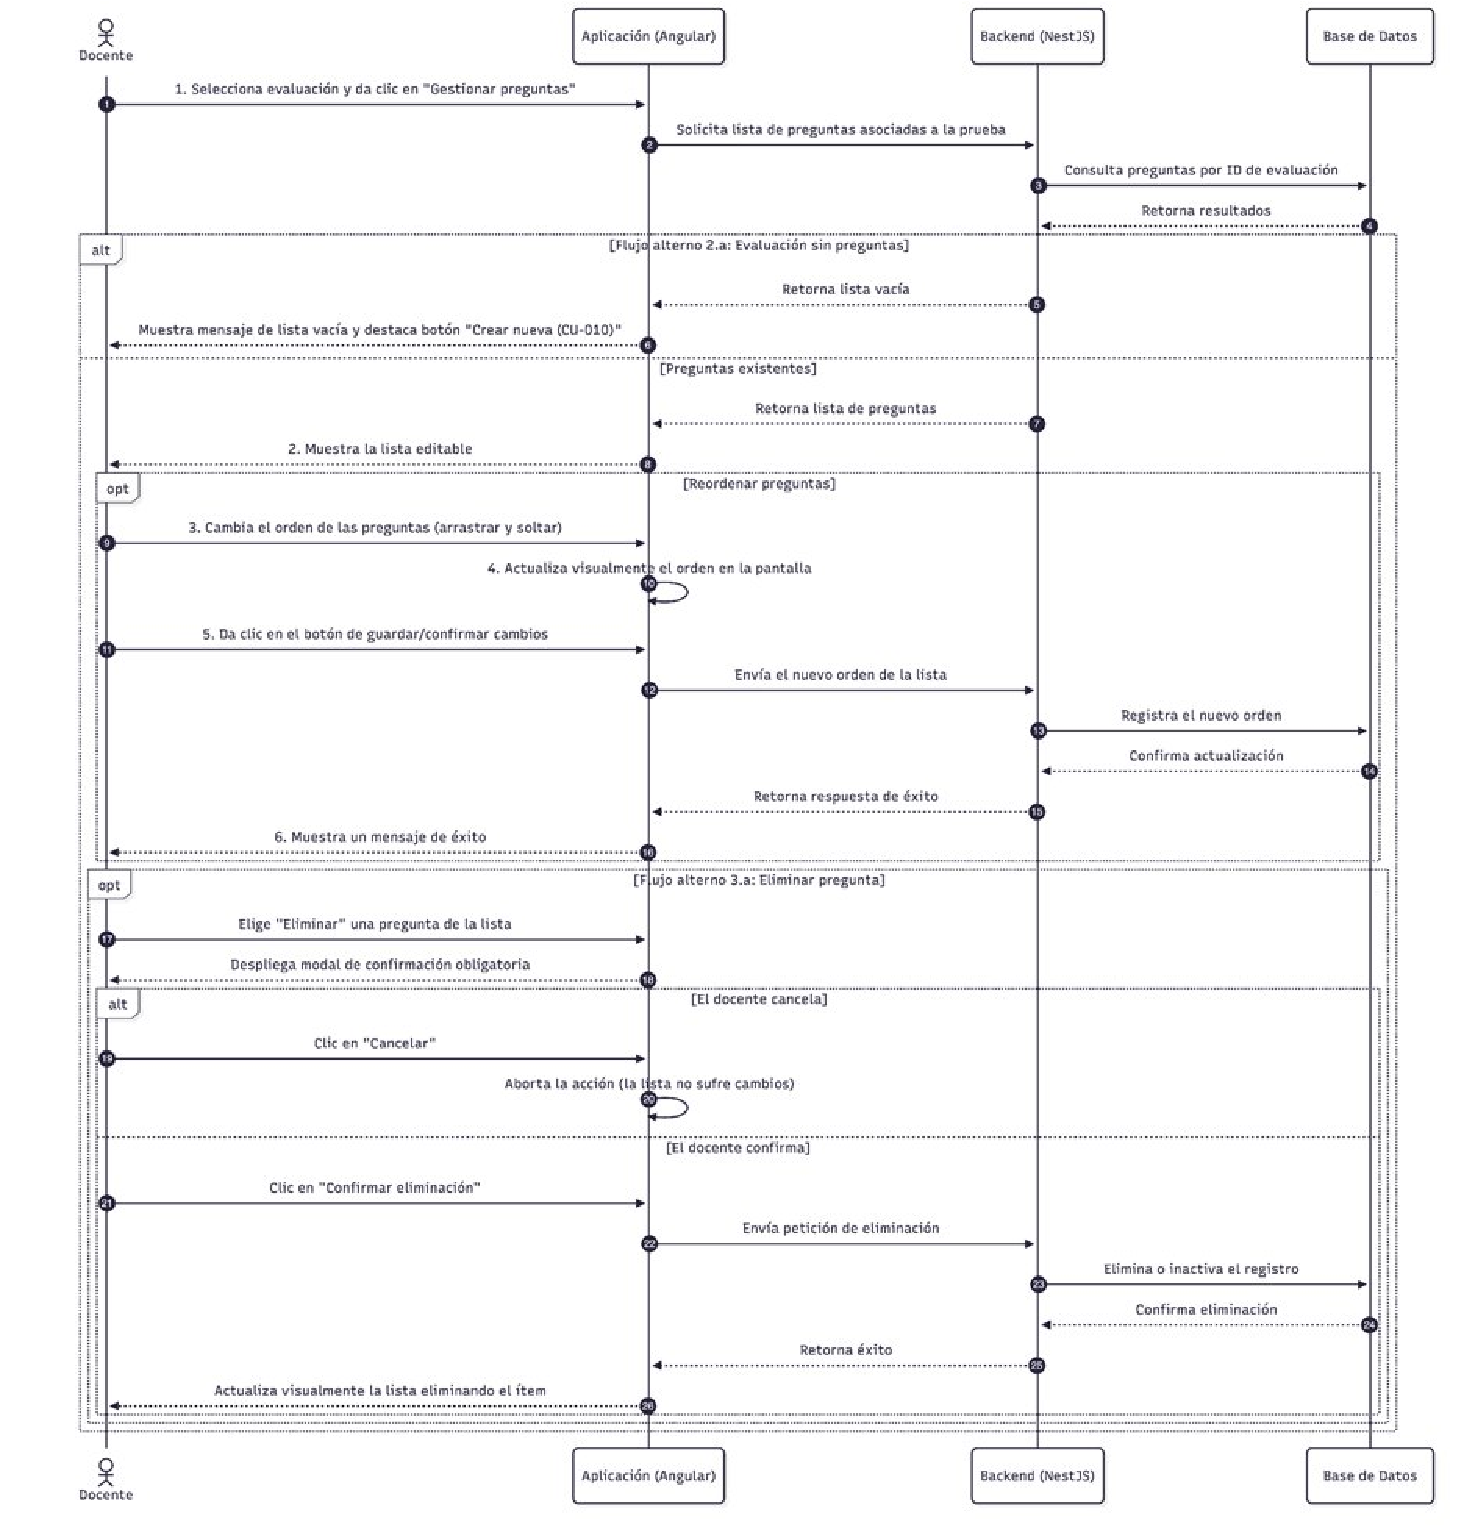
\includegraphics[width=0.92\textwidth,height=10cm,keepaspectratio]{figuras/seq_organizar_preguntas.pdf}}\\\hline
\rowcolor{tabhead2}\multicolumn{4}{|c|}{\textbf{Interfaz de usuario}}\\\hline
\multicolumn{4}{|c|}{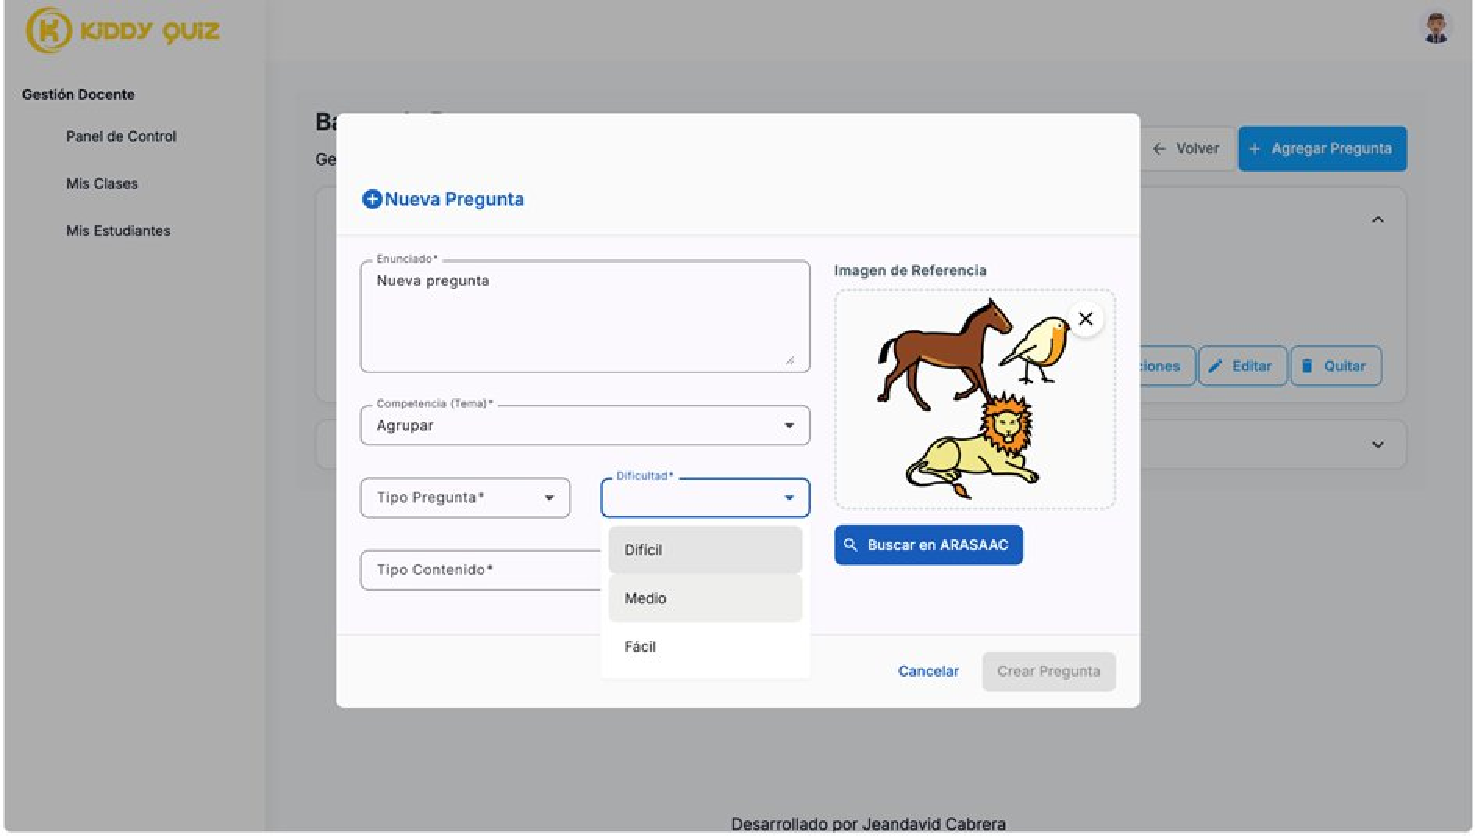
\includegraphics[width=0.92\textwidth,height=8cm,keepaspectratio]{figuras/ui_nueva_pregunta.pdf}}\\\hline
Comentarios: & \multicolumn{3}{X|}{Se sugiere incluir botones de navegación amigables para moverse entre la lista de preguntas y la configuración general. Esta gestión se beneficia directamente de tener un control de versiones o historial de cambios.}\\\hline
\end{tabularx}
\end{footnotesize}
\fuenteautor
\end{table}

\begin{table}[H]
\centering
\caption{Caso de uso ``Configurar contenido''.}
\label{tab:cu_config}
\begin{footnotesize}
\renewcommand{\arraystretch}{1.25}
\begin{tabularx}{\textwidth}{|>{\bfseries}L{2.6cm}|X|>{\bfseries}L{2.4cm}|X|}
\hline
\rowcolor{tabhead}\multicolumn{4}{|c|}{\tabhead{Caso de uso ``Configurar contenido''}}\\\hline
Código: & CU-010 & Actores: & Docente\\\hline
Objetivo: & \multicolumn{3}{X|}{Permitir al docente crear preguntas estructuradas para una evaluación, definiendo el enunciado, el formato y las opciones de respuesta válidas.}\\\hline
Resumen: & \multicolumn{3}{X|}{El docente selecciona el tipo de pregunta (opción múltiple, verdadero/falso, etc.), redacta el enunciado y configura las opciones indicando cuál es la correcta. El sistema valida la integridad de la pregunta y la guarda.}\\\hline
Tipo: & \multicolumn{3}{X|}{Principal}\\\hline
Dependencias: & \multicolumn{3}{X|}{\textbf{Invoca a:} CU-011 (Soporte multimedia en preguntas). \par \textbf{Depende de:} Evaluación existente e Interfaz de edición docente.}\\\hline
Precondición: & \multicolumn{3}{X|}{El docente debe estar autenticado, haber seleccionado una evaluación previamente creada y encontrarse dentro de la interfaz de gestión de preguntas (CU-009).}\\\hline
Postcondición: & \multicolumn{3}{X|}{La nueva pregunta, junto con su enunciado, tipo y estructura de respuestas, se registra exitosamente en la base de datos asociada al ID de la evaluación.}\\\hline
[Importancia]: & \multicolumn{3}{X|}{Muy alta -- Permite generar contenido pedagógico evaluativo y asegurar que el sistema califique automáticamente.}\\\hline
\rowcolor{tabhead2}\multicolumn{4}{|c|}{\textbf{Flujo normal de eventos}}\\\hline
\rowcolor{tabhead2}\multicolumn{2}{|>{\columncolor{tabhead2}}c|}{\textbf{Acción del actor}} & \multicolumn{2}{>{\columncolor{tabhead2}}c|}{\textbf{Respuesta del sistema}}\\\hline
\multicolumn{2}{|X|}{1.~El docente da clic en la opción para agregar un nuevo ítem evaluativo.} & \multicolumn{2}{X|}{}\\\hline
\multicolumn{2}{|X|}{} & \multicolumn{2}{X|}{2.~El sistema provee un formulario con un campo de texto enriquecido para el enunciado y un selector de tipo de pregunta.}\\\hline
\multicolumn{2}{|X|}{3.~El docente ingresa el enunciado y selecciona el formato (múltiple, V/F o corta).} & \multicolumn{2}{X|}{}\\\hline
\multicolumn{2}{|X|}{} & \multicolumn{2}{X|}{4.~El sistema adapta dinámicamente los campos inferiores para ingresar las opciones de respuesta.}\\\hline
\multicolumn{2}{|X|}{5.~El docente llena las opciones y marca explícitamente cuál es la correcta.} & \multicolumn{2}{X|}{}\\\hline
\multicolumn{2}{|X|}{6.~El docente hace clic en ``Guardar''.} & \multicolumn{2}{X|}{}\\\hline
\multicolumn{2}{|X|}{} & \multicolumn{2}{X|}{7.~El sistema verifica la información y registra la pregunta en la base de datos vinculada a la evaluación.}\\\hline
\multicolumn{2}{|X|}{} & \multicolumn{2}{X|}{8.~La aplicación actualiza la vista mostrando la nueva pregunta en la lista.}\\\hline
\rowcolor{tabhead2}\multicolumn{4}{|c|}{\textbf{Flujo alterno}}\\\hline
\multicolumn{4}{|X|}{\textbf{7.a.} Si el docente olvida marcar al menos una respuesta como correcta, el sistema aplica una validación automática que impide guardar la pregunta y resalta el error en pantalla. \par \textbf{5.a.} Antes de guardar, el docente puede seleccionar la opción de ``Vista previa'' y el sistema renderizará la pregunta tal como la verá el estudiante.}\\\hline
\rowcolor{tabhead2}\multicolumn{4}{|c|}{\textbf{Diagrama de secuencia}}\\\hline
\multicolumn{4}{|c|}{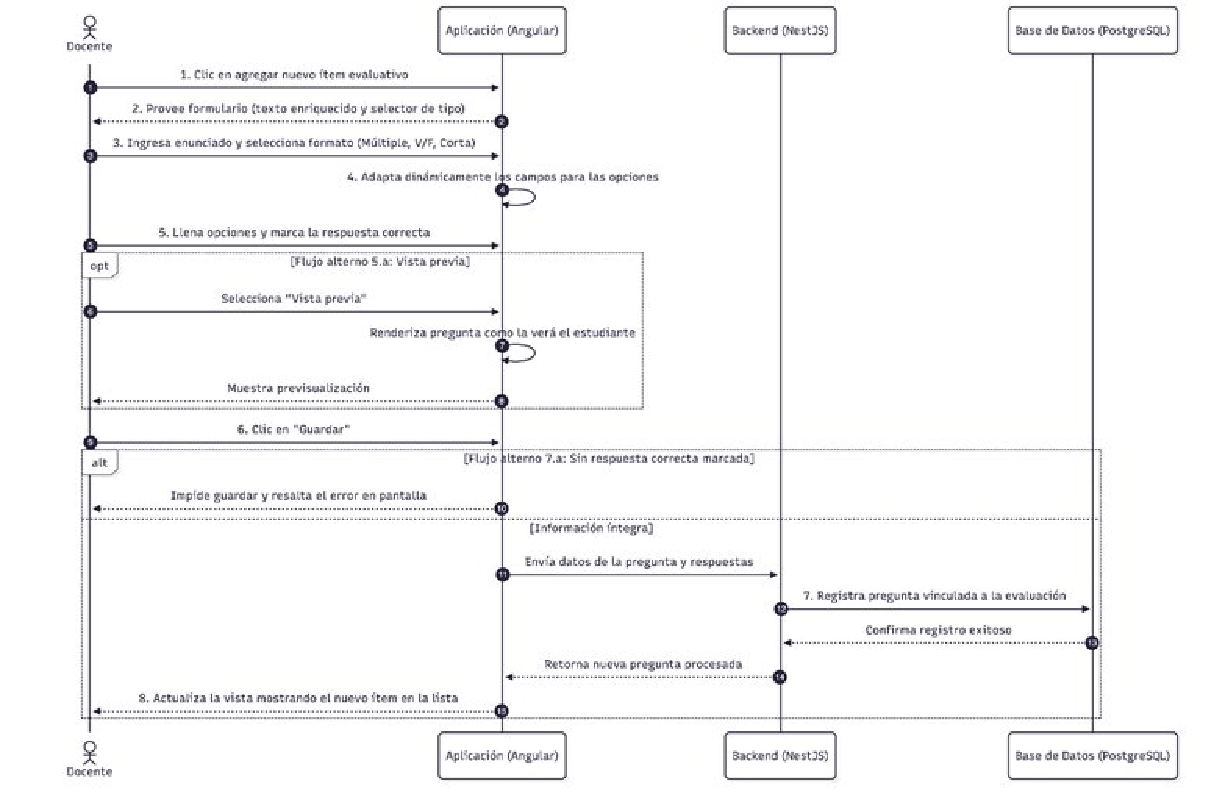
\includegraphics[width=0.92\textwidth,height=10cm,keepaspectratio]{figuras/seq_configurar_contenido.pdf}}\\\hline
\rowcolor{tabhead2}\multicolumn{4}{|c|}{\textbf{Interfaz de usuario}}\\\hline
\multicolumn{4}{|c|}{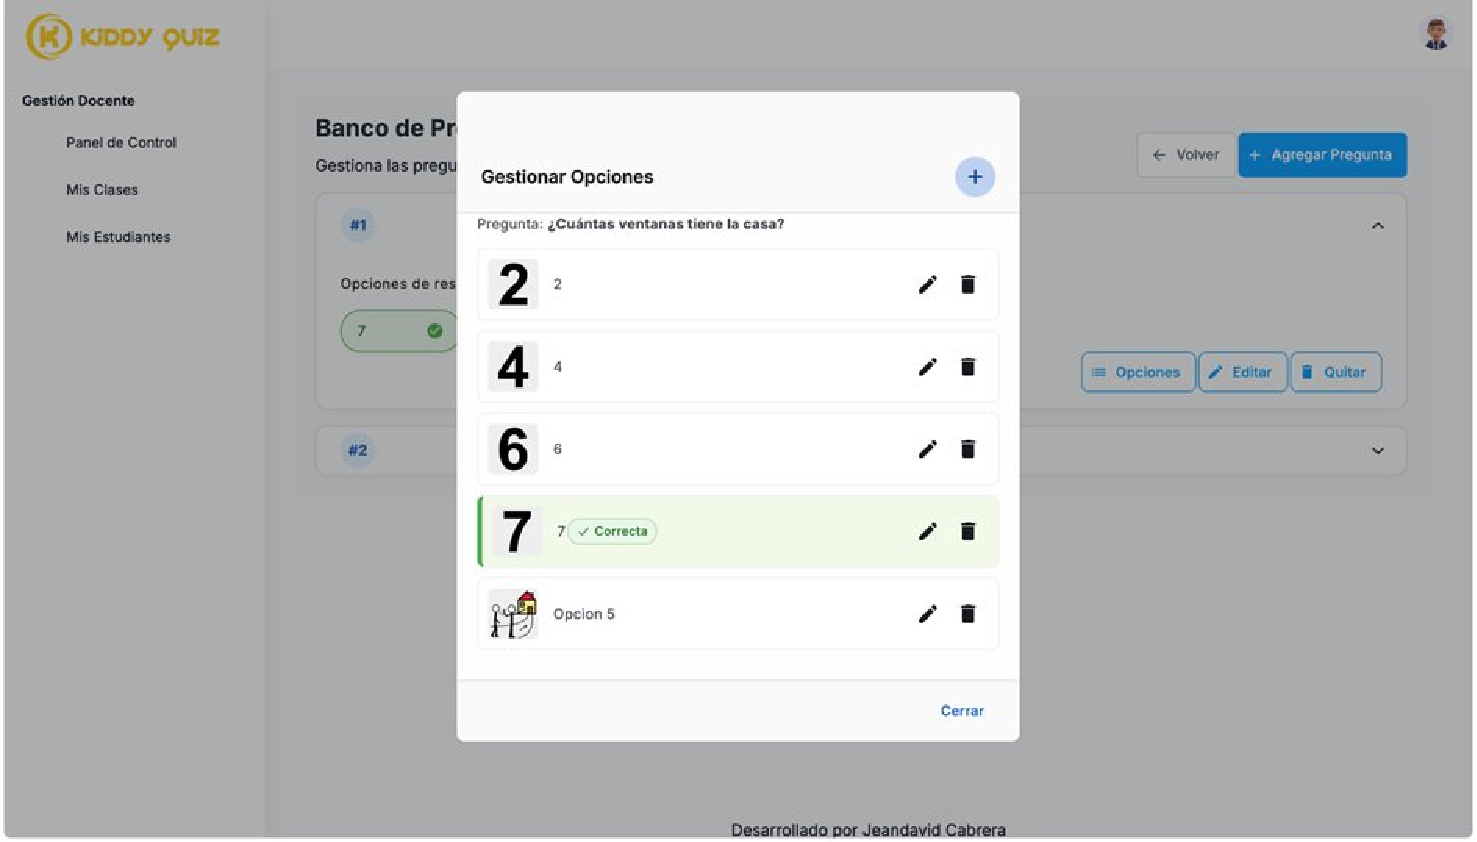
\includegraphics[width=0.92\textwidth,height=8cm,keepaspectratio]{figuras/ui_gestionar_opciones.pdf}}\\\hline
Comentarios: & \multicolumn{3}{X|}{La validación de la respuesta correcta es crítica para que el motor de evaluación (CU-004) pueda funcionar. El campo de enunciado debe soportar texto enriquecido para dar formato a la lectura.}\\\hline
\end{tabularx}
\end{footnotesize}
\fuenteautor
\end{table}

\begin{table}[H]
\centering
\caption{Caso de uso ``Adjuntar archivos multimedia''.}
\label{tab:cu_multimedia}
\begin{footnotesize}
\renewcommand{\arraystretch}{1.25}
\begin{tabularx}{\textwidth}{|>{\bfseries}L{2.6cm}|X|>{\bfseries}L{2.4cm}|X|}
\hline
\rowcolor{tabhead}\multicolumn{4}{|c|}{\tabhead{Caso de uso ``Adjuntar archivos multimedia''}}\\\hline
Código: & CU-011 & Actores: & Docente\\\hline
Objetivo: & \multicolumn{3}{X|}{Permitir al docente cargar e integrar recursos multimedia (imágenes, GIFs o videos) en las preguntas para enriquecer visualmente la evaluación.}\\\hline
Resumen: & \multicolumn{3}{X|}{El docente sube un archivo multimedia al editor de preguntas. El sistema valida la extensión y el tamaño, muestra una vista previa y vincula la URL del archivo a la pregunta en la posición elegida.}\\\hline
Tipo: & \multicolumn{3}{X|}{Secundario (Extensión de CU-010)}\\\hline
Dependencias: & \multicolumn{3}{X|}{\textbf{Invoca a:} ninguno directamente; es una extensión de CU-010. \par \textbf{Depende de:} Módulo de creación de preguntas y el Sistema de almacenamiento de archivos multimedia.}\\\hline
Precondición: & \multicolumn{3}{X|}{El docente debe estar autenticado y encontrarse dentro de la interfaz de creación o edición de una pregunta específica (CU-010).}\\\hline
Postcondición: & \multicolumn{3}{X|}{El archivo multimedia se procesa, se guarda de forma segura, y su ruta de acceso (URL) se vincula a la pregunta correspondiente en la base de datos, respetando la posición configurada por el docente.}\\\hline
[Importancia]: & \multicolumn{3}{X|}{Alta -- Aumenta la comprensión en alumnos con diferentes estilos de aprendizaje.}\\\hline
\rowcolor{tabhead2}\multicolumn{4}{|c|}{\textbf{Flujo normal de eventos}}\\\hline
\rowcolor{tabhead2}\multicolumn{2}{|>{\columncolor{tabhead2}}c|}{\textbf{Acción del actor}} & \multicolumn{2}{>{\columncolor{tabhead2}}c|}{\textbf{Respuesta del sistema}}\\\hline
\multicolumn{2}{|X|}{1.~El docente interactúa con la zona de carga de archivos (tipo \textit{Drag \& Drop} o con botón de selección) en el editor de preguntas.} & \multicolumn{2}{X|}{}\\\hline
\multicolumn{2}{|X|}{} & \multicolumn{2}{X|}{2.~El sistema habilita la selección o recepción del recurso multimedia.}\\\hline
\multicolumn{2}{|X|}{3.~El docente selecciona un archivo e indica la posición deseada (arriba o abajo del enunciado).} & \multicolumn{2}{X|}{}\\\hline
\multicolumn{2}{|X|}{} & \multicolumn{2}{X|}{4.~El sistema valida estrictamente que la extensión sea \texttt{.jpg}, \texttt{.png}, \texttt{.gif} o \texttt{.mp4} y que no exceda el límite de tamaño.}\\\hline
\multicolumn{2}{|X|}{} & \multicolumn{2}{X|}{5.~Al cargar el archivo con éxito, la interfaz genera y muestra una vista previa integrada en tiempo real.}\\\hline
\multicolumn{2}{|X|}{6.~El docente finaliza y guarda la pregunta.} & \multicolumn{2}{X|}{}\\\hline
\multicolumn{2}{|X|}{} & \multicolumn{2}{X|}{7.~El sistema almacena el recurso y vincula su URL a la pregunta en la base de datos.}\\\hline
\rowcolor{tabhead2}\multicolumn{4}{|c|}{\textbf{Flujo alterno}}\\\hline
\multicolumn{4}{|X|}{\textbf{4.a.\ Formato no soportado:} si el archivo no es \texttt{.jpg}, \texttt{.png}, \texttt{.gif} ni \texttt{.mp4}, el sistema rechaza la carga y muestra un error indicando los formatos válidos. \par \textbf{4.b.\ Exceso de tamaño:} si el archivo supera el límite máximo permitido (ej. 2~MB para imágenes/GIFs o 10~MB para videos), el sistema advierte sobre el límite y detiene la carga para asegurar el rendimiento del servidor.}\\\hline
\rowcolor{tabhead2}\multicolumn{4}{|c|}{\textbf{Diagrama de secuencia}}\\\hline
\multicolumn{4}{|c|}{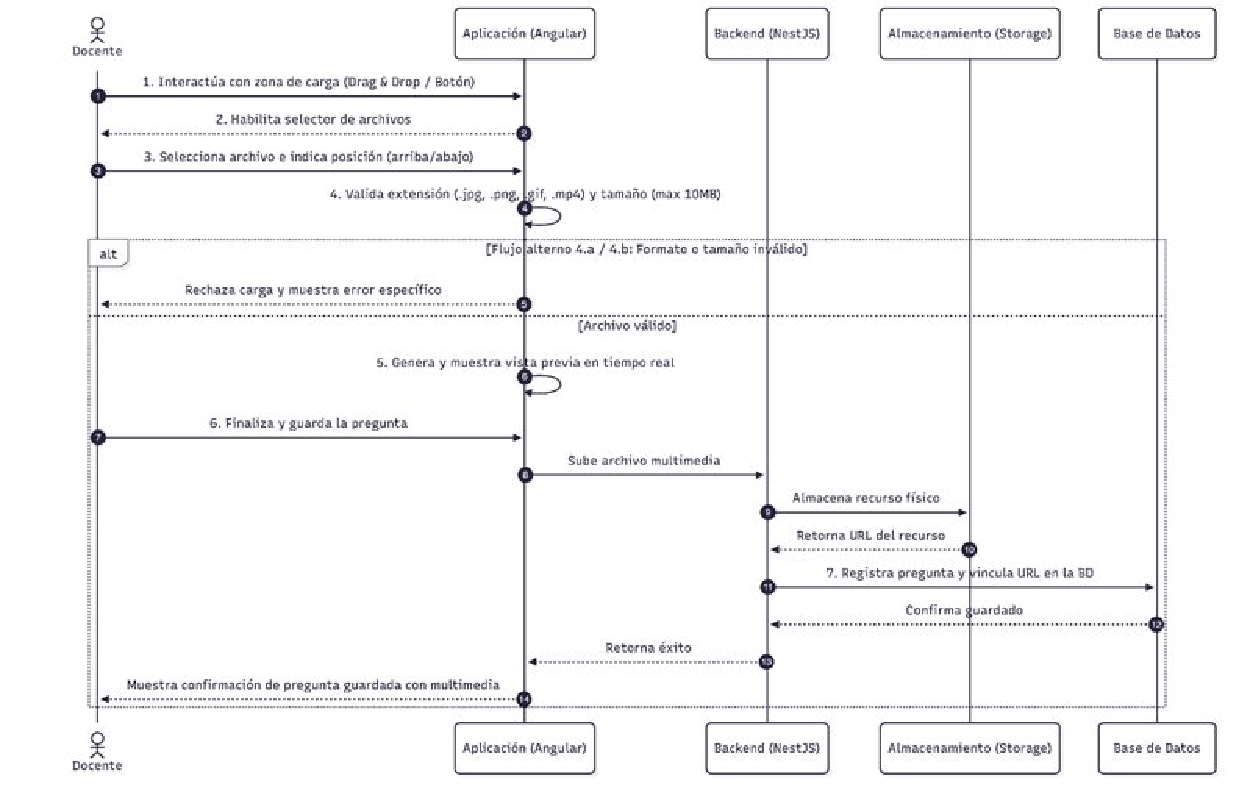
\includegraphics[width=0.92\textwidth,height=10cm,keepaspectratio]{figuras/seq_adjuntar_multimedia.pdf}}\\\hline
\rowcolor{tabhead2}\multicolumn{4}{|c|}{\textbf{Interfaz de usuario}}\\\hline
\multicolumn{4}{|c|}{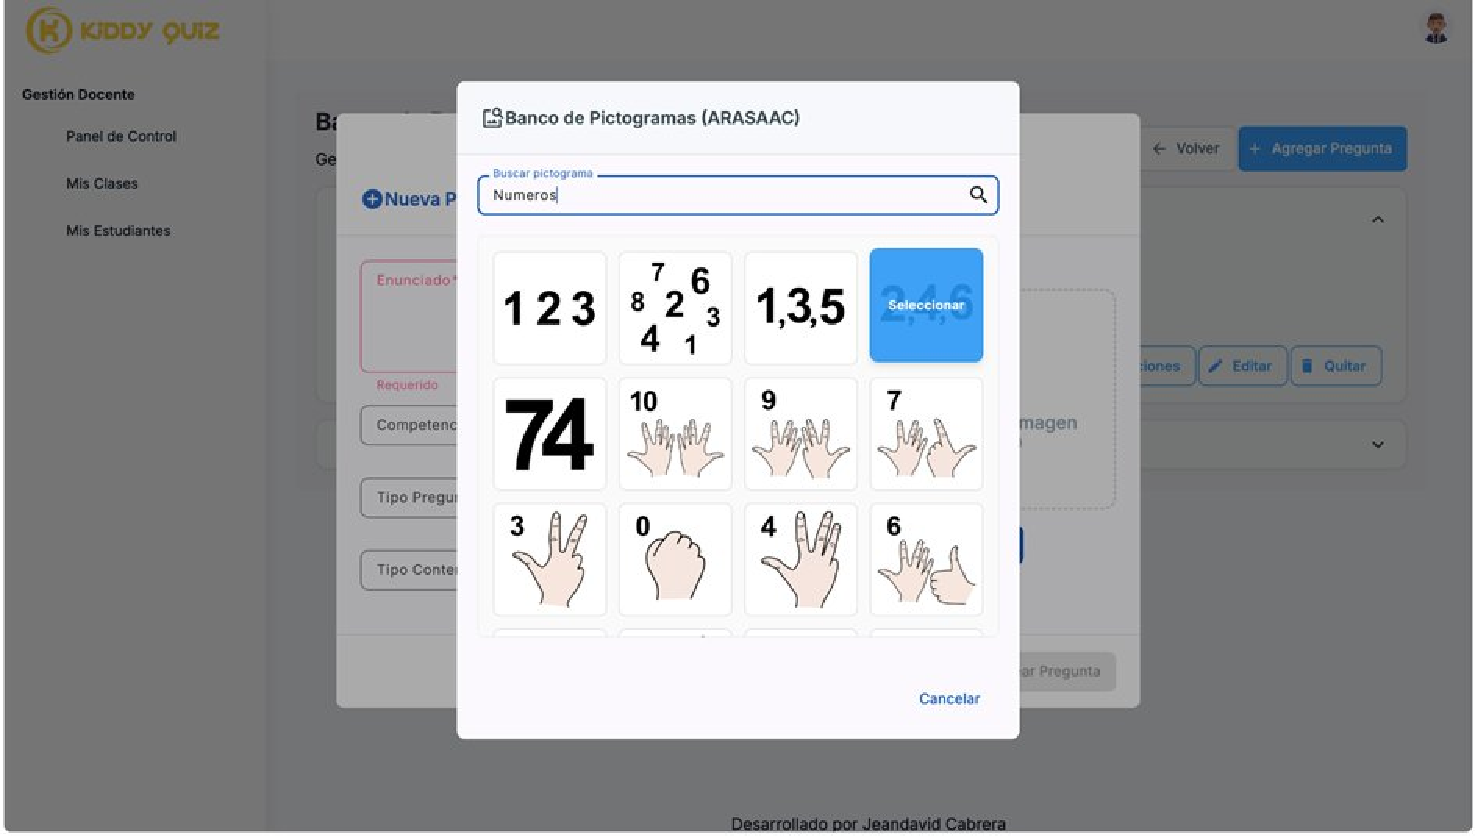
\includegraphics[width=0.92\textwidth,height=8cm,keepaspectratio]{figuras/ui_arasaac_pictogramas.pdf}}\\\hline
Comentarios: & \multicolumn{3}{X|}{Se debe verificar la compatibilidad con dispositivos móviles y limitar el tamaño de los archivos para asegurar un buen rendimiento. Los recursos deben renderizarse de forma responsiva en el panel del estudiante, adaptando su tamaño a las pantallas móviles sin deformarse.}\\\hline
\end{tabularx}
\end{footnotesize}
\fuenteautor
\end{table}

\begin{table}[H]
\centering
\caption{Caso de uso ``Consultar alumnos''.}
\label{tab:cu_alumnos}
\begin{footnotesize}
\renewcommand{\arraystretch}{1.25}
\begin{tabularx}{\textwidth}{|>{\bfseries}L{2.6cm}|X|>{\bfseries}L{2.4cm}|X|}
\hline
\rowcolor{tabhead}\multicolumn{4}{|c|}{\tabhead{Caso de uso ``Consultar alumnos''}}\\\hline
Código: & CU-012 & Actores: & Docente\\\hline
Objetivo: & \multicolumn{3}{X|}{Visualizar una lista completa y filtrable de los alumnos registrados y vinculados al docente, organizados por curso o grupo, para llevar un seguimiento de su estado en la plataforma.}\\\hline
Resumen: & \multicolumn{3}{X|}{El docente accede a la sección de estudiantes; el sistema consulta la base de datos y despliega una tabla con los alumnos del docente (nombre, curso, estado). El sistema permite filtrar resultados por nombre mediante un buscador.}\\\hline
Tipo: & \multicolumn{3}{X|}{Principal}\\\hline
Dependencias: & \multicolumn{3}{X|}{\textbf{Invoca a:} CU-013 (Visualización de resultados generales y por prueba, al hacer clic en un estudiante específico). \par \textbf{Depende de:} Módulo de registro, Asociación alumno-docente y la Base de datos de usuarios.}\\\hline
Precondición: & \multicolumn{3}{X|}{El docente debe haber iniciado sesión exitosamente en el sistema. Debe existir al menos un estudiante registrado y vinculado correctamente al código único de este docente (CU-002).}\\\hline
Postcondición: & \multicolumn{3}{X|}{El sistema despliega correctamente la lista de alumnos según los filtros aplicados. El docente obtiene una vista clara de sus clases y el sistema queda a la espera de que seleccione un estudiante para consultar su rendimiento.}\\\hline
[Importancia]: & \multicolumn{3}{X|}{Alta -- Permite acceder rápidamente al seguimiento individual.}\\\hline
\rowcolor{tabhead2}\multicolumn{4}{|c|}{\textbf{Flujo normal de eventos}}\\\hline
\rowcolor{tabhead2}\multicolumn{2}{|>{\columncolor{tabhead2}}c|}{\textbf{Acción del actor}} & \multicolumn{2}{>{\columncolor{tabhead2}}c|}{\textbf{Respuesta del sistema}}\\\hline
\multicolumn{2}{|X|}{1.~El docente accede a la sección de gestión de estudiantes.} & \multicolumn{2}{X|}{}\\\hline
\multicolumn{2}{|X|}{} & \multicolumn{2}{X|}{2.~El sistema identifica el ID del docente y consulta la base de datos buscando únicamente a los alumnos vinculados a él.}\\\hline
\multicolumn{2}{|X|}{} & \multicolumn{2}{X|}{3.~La aplicación muestra una lista o tabla organizada por curso, indicando obligatoriamente: nombre completo, curso/grupo y estado (activo/inactivo).}\\\hline
\multicolumn{2}{|X|}{} & \multicolumn{2}{X|}{4.~El sistema muestra un indicador o contador del total de alumnos inscritos por cada grupo.}\\\hline
\multicolumn{2}{|X|}{5.~El docente utiliza el buscador ingresando el nombre de un alumno específico.} & \multicolumn{2}{X|}{}\\\hline
\multicolumn{2}{|X|}{} & \multicolumn{2}{X|}{6.~El sistema filtra los resultados en tiempo real y muestra las coincidencias exactas o parciales en la lista.}\\\hline
\multicolumn{2}{|X|}{7.~El docente selecciona a un estudiante de la lista.} & \multicolumn{2}{X|}{}\\\hline
\multicolumn{2}{|X|}{} & \multicolumn{2}{X|}{8.~El sistema redirige a la vista de perfil de rendimiento del estudiante seleccionado (CU-013).}\\\hline
\rowcolor{tabhead2}\multicolumn{4}{|c|}{\textbf{Flujo alterno}}\\\hline
\multicolumn{4}{|X|}{\textbf{3.a.} Si el docente aún no tiene alumnos vinculados, el sistema muestra un mensaje indicando que no hay estudiantes registrados y le recuerda su código de vinculación para que lo comparta. \par \textbf{6.a.} Si la búsqueda no arroja coincidencias, el sistema muestra un mensaje de ``No se encontraron alumnos con ese nombre'' y permite limpiar el buscador.}\\\hline
\rowcolor{tabhead2}\multicolumn{4}{|c|}{\textbf{Diagrama de secuencia}}\\\hline
\multicolumn{4}{|c|}{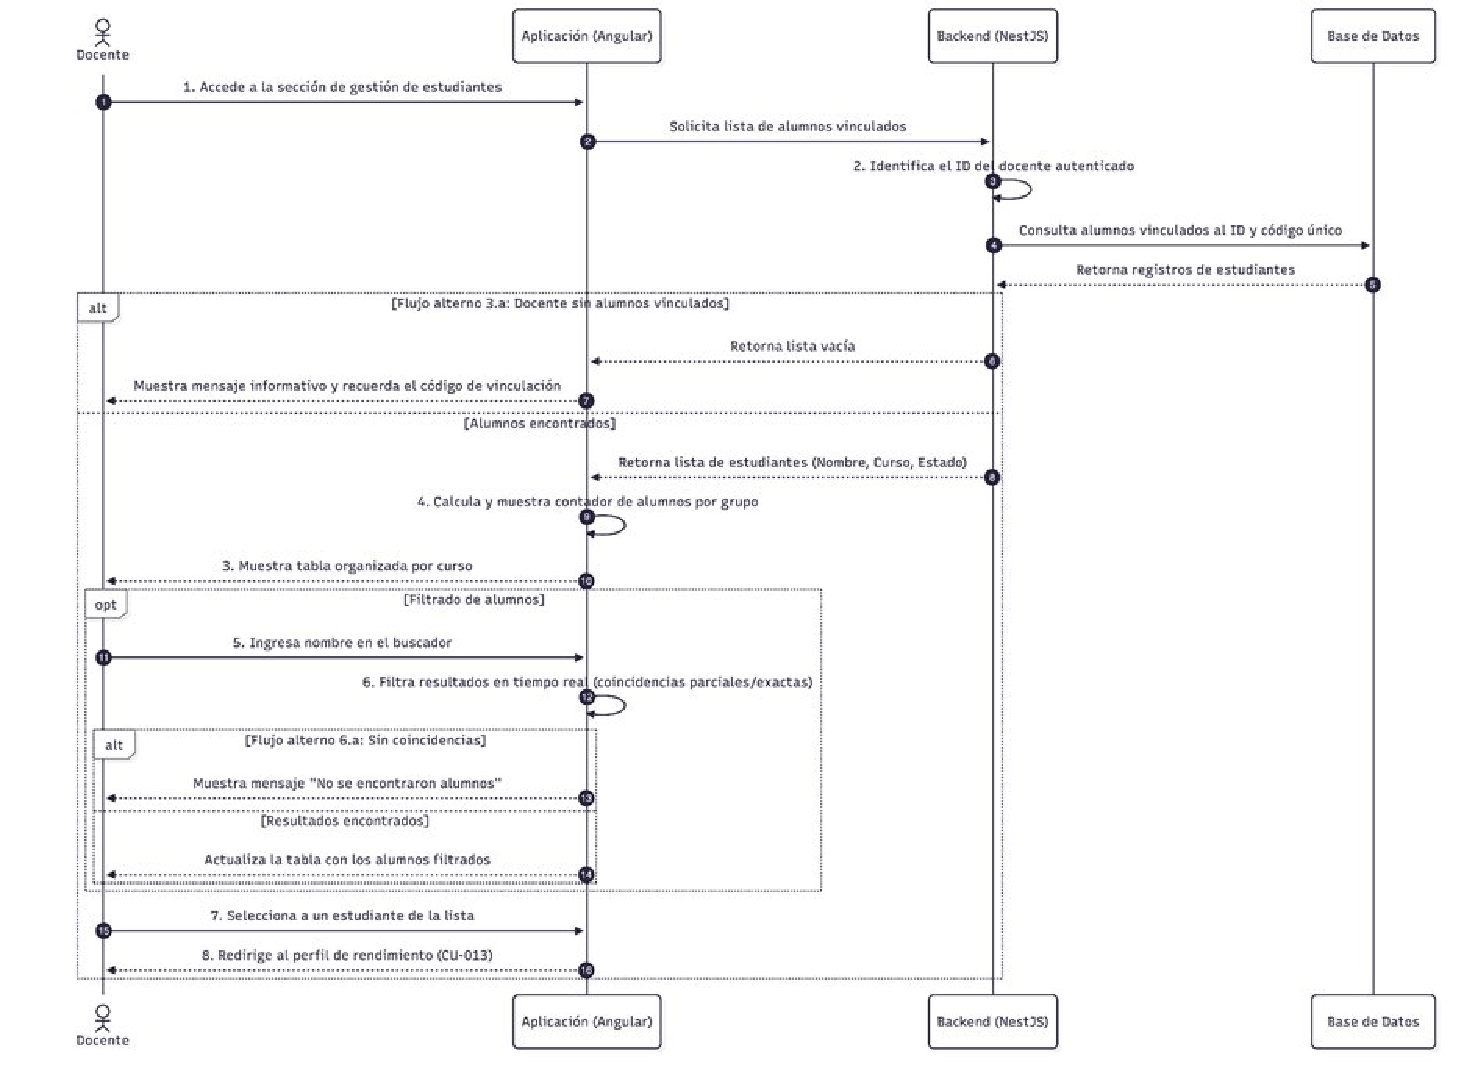
\includegraphics[width=0.92\textwidth,height=10cm,keepaspectratio]{figuras/seq_consultar_alumnos.pdf}}\\\hline
\rowcolor{tabhead2}\multicolumn{4}{|c|}{\textbf{Interfaz de usuario}}\\\hline
\multicolumn{4}{|c|}{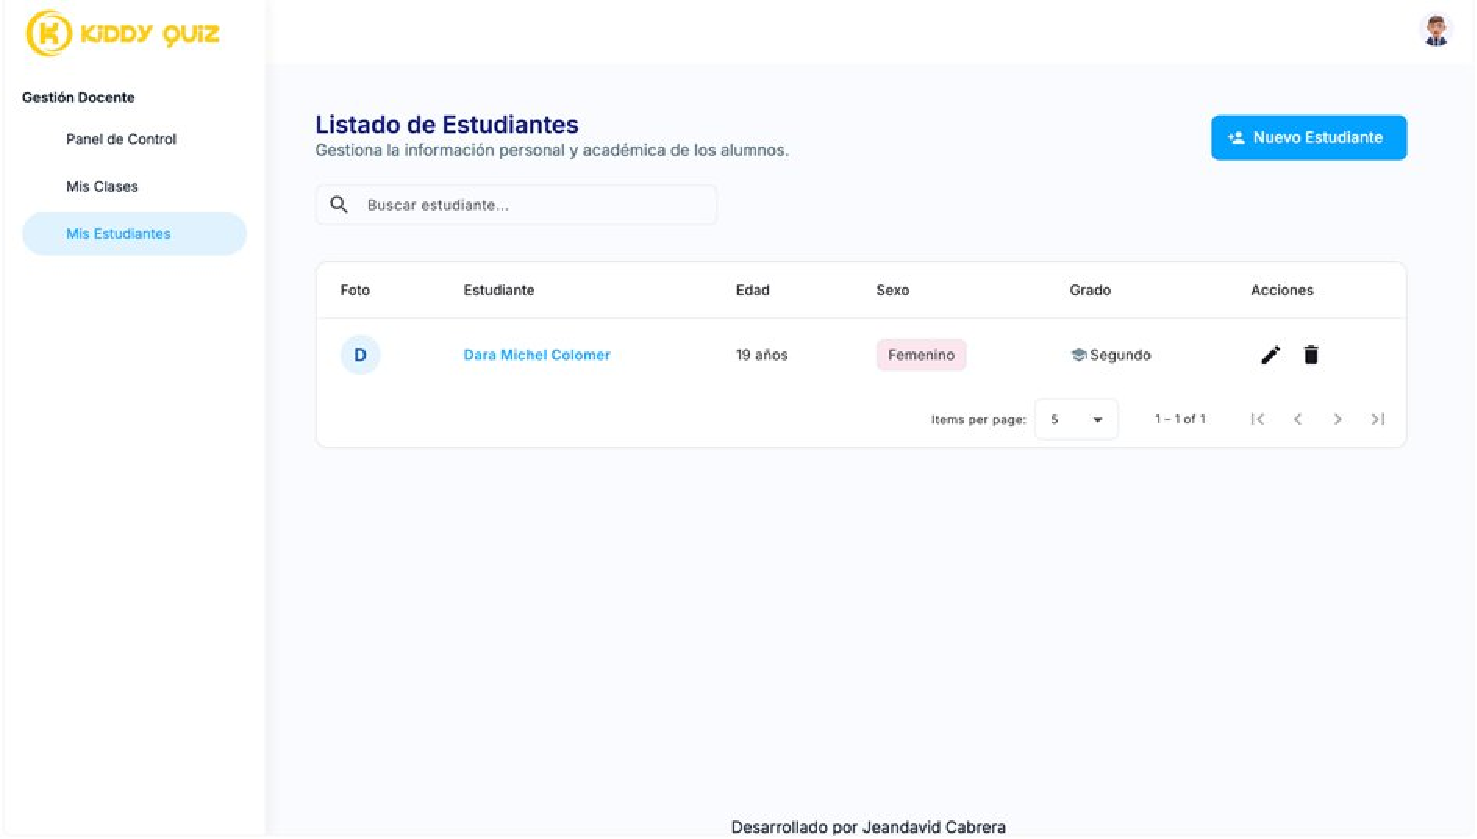
\includegraphics[width=0.92\textwidth,height=8cm,keepaspectratio]{figuras/ui_listado_estudiantes.pdf}}\\\hline
Comentarios: & \multicolumn{3}{X|}{La interfaz debe ser limpia y responsiva, garantizando que la tabla o lista se adapte correctamente a pantallas de dispositivos móviles sin perder columnas de información.}\\\hline
\end{tabularx}
\end{footnotesize}
\fuenteautor
\end{table}

\begin{table}[H]
\centering
\caption{Caso de uso ``Analizar calificaciones''.}
\label{tab:cu_analizar}
\begin{footnotesize}
\renewcommand{\arraystretch}{1.25}
\begin{tabularx}{\textwidth}{|>{\bfseries}L{2.6cm}|X|>{\bfseries}L{2.4cm}|X|}
\hline
\rowcolor{tabhead}\multicolumn{4}{|c|}{\tabhead{Caso de uso ``Analizar calificaciones''}}\\\hline
Código: & CU-013 & Actores: & Docente\\\hline
Objetivo: & \multicolumn{3}{X|}{Acceder al perfil académico de un estudiante desde el listado general para visualizar su promedio global y el desglose de resultados por cada evaluación realizada.}\\\hline
Resumen: & \multicolumn{3}{X|}{El docente selecciona a un estudiante para evaluar su progreso individual. El sistema calcula y muestra el promedio acumulado junto con una lista detallada de cada prueba completada (puntaje, fecha, duración), utilizando colores o íconos para destacar el nivel de desempeño.}\\\hline
Tipo: & \multicolumn{3}{X|}{Principal}\\\hline
Dependencias: & \multicolumn{3}{X|}{\textbf{Invoca a:} CU-014 (Curva de mejora individual) y CU-015 (Exportación de resultados a Excel). \par \textbf{Depende de:} Evaluaciones realizadas, Motor de análisis de resultados y acceso desde el listado de alumnos (CU-012).}\\\hline
Precondición: & \multicolumn{3}{X|}{El docente debe estar autenticado, encontrarse en la lista de alumnos (CU-012) y seleccionar a un estudiante específico. El estudiante debe haber completado al menos una evaluación previamente para que existan datos que analizar.}\\\hline
Postcondición: & \multicolumn{3}{X|}{El sistema presenta en pantalla el promedio general del estudiante y los resultados desglosados, mostrando explícitamente el puntaje, la fecha y la duración.}\\\hline
[Importancia]: & \multicolumn{3}{X|}{Muy alta -- Fundamental para evaluar el progreso del alumno, identificar su nivel de desempeño y compararlo dentro del grupo escolar.}\\\hline
\rowcolor{tabhead2}\multicolumn{4}{|c|}{\textbf{Flujo normal de eventos}}\\\hline
\rowcolor{tabhead2}\multicolumn{2}{|>{\columncolor{tabhead2}}c|}{\textbf{Acción del actor}} & \multicolumn{2}{>{\columncolor{tabhead2}}c|}{\textbf{Respuesta del sistema}}\\\hline
\multicolumn{2}{|X|}{1.~El docente hace clic en un alumno específico desde la pantalla de ``Lista de alumnos'' (CU-012).} & \multicolumn{2}{X|}{}\\\hline
\multicolumn{2}{|X|}{} & \multicolumn{2}{X|}{2.~El sistema consulta el historial de evaluaciones completadas por el estudiante seleccionado.}\\\hline
\multicolumn{2}{|X|}{} & \multicolumn{2}{X|}{3.~El sistema calcula el promedio general acumulado del estudiante.}\\\hline
\multicolumn{2}{|X|}{} & \multicolumn{2}{X|}{4.~La aplicación muestra el perfil del estudiante destacando visualmente el promedio global calculado.}\\\hline
\multicolumn{2}{|X|}{} & \multicolumn{2}{X|}{5.~El sistema despliega el desglose de cada evaluación, mostrando de forma obligatoria: el puntaje obtenido, la fecha de realización y la duración (tiempo empleado).}\\\hline
\multicolumn{2}{|X|}{} & \multicolumn{2}{X|}{6.~El sistema aplica colores o íconos de desempeño a cada resultado (ej. verde para aprobado, rojo para bajo rendimiento) para facilitar la interpretación visual rápida.}\\\hline
\multicolumn{2}{|X|}{7.~El docente utiliza los controles de la interfaz para ordenar los resultados detallados (por ejemplo, por fecha o por puntaje).} & \multicolumn{2}{X|}{}\\\hline
\multicolumn{2}{|X|}{} & \multicolumn{2}{X|}{8.~El sistema actualiza dinámicamente el orden de la lista en pantalla.}\\\hline
\rowcolor{tabhead2}\multicolumn{4}{|c|}{\textbf{Flujo alterno}}\\\hline
\multicolumn{4}{|X|}{\textbf{2.a.} Si el estudiante aún no ha completado ninguna evaluación, el sistema muestra el promedio general como ``0'' o ``N/A'' y despliega un mensaje amigable indicando que no hay registros históricos disponibles. \par \textbf{3.a.} Si ocurre un error de conexión al consultar la base de datos, el sistema muestra una alerta de error y sugiere recargar el perfil del alumno.}\\\hline
\rowcolor{tabhead2}\multicolumn{4}{|c|}{\textbf{Diagrama de secuencia}}\\\hline
\multicolumn{4}{|c|}{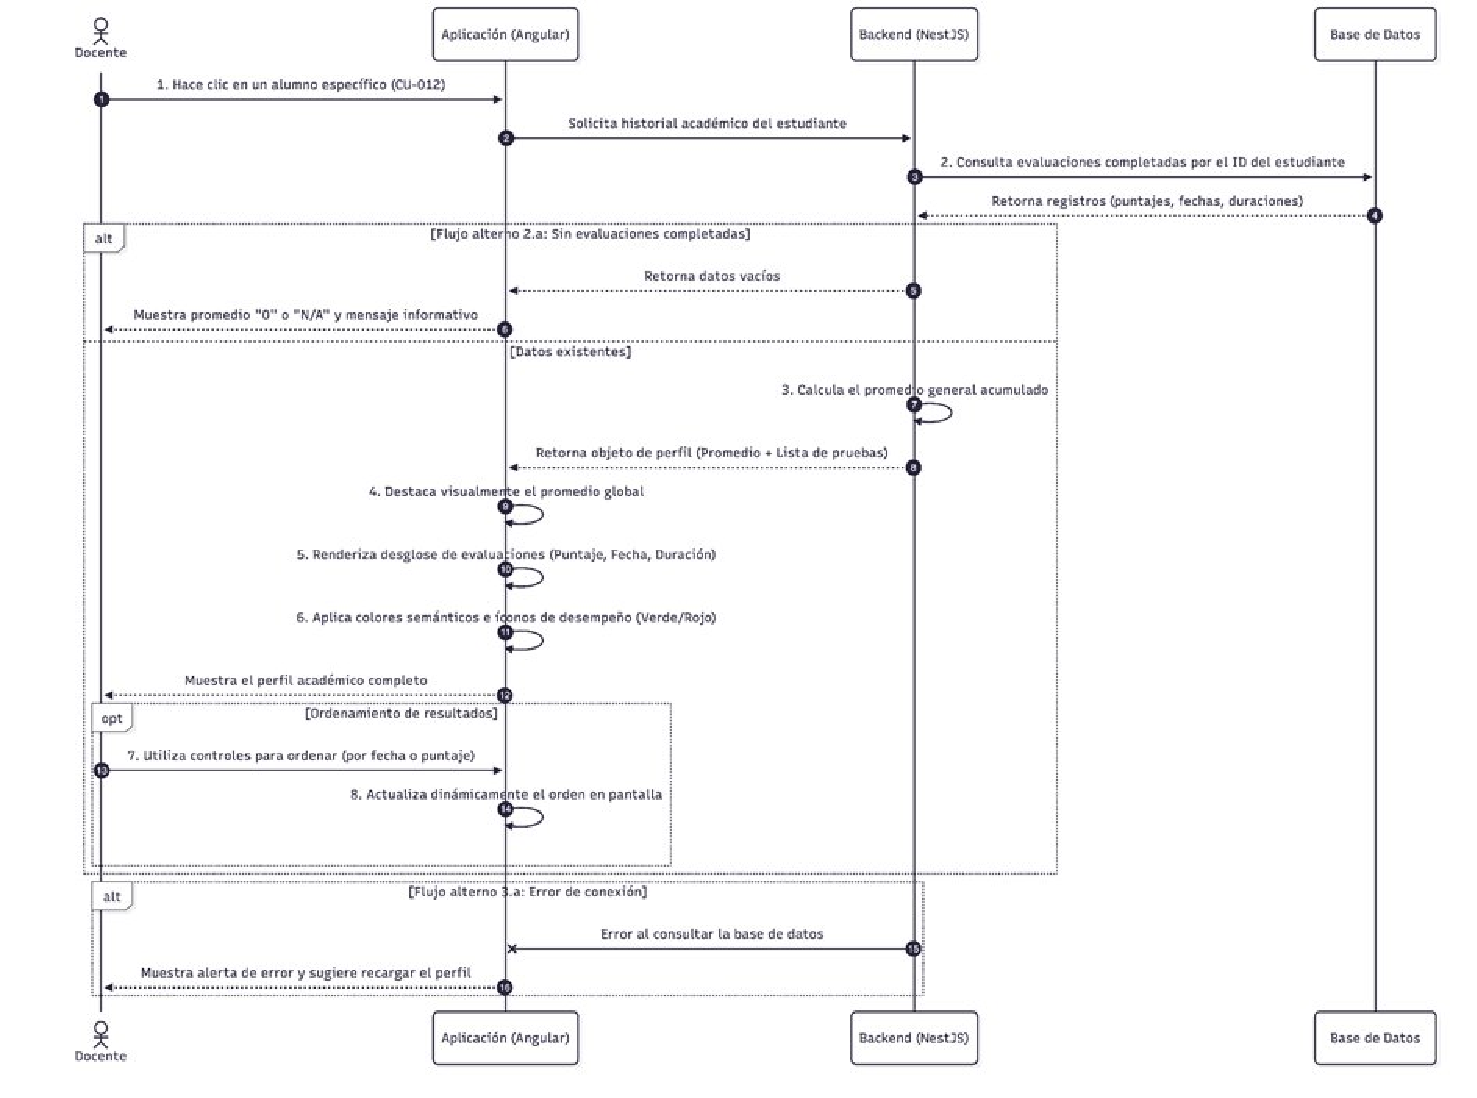
\includegraphics[width=0.92\textwidth,height=10cm,keepaspectratio]{figuras/seq_analizar_calificaciones.pdf}}\\\hline
\rowcolor{tabhead2}\multicolumn{4}{|c|}{\textbf{Interfaz de usuario}}\\\hline
\multicolumn{4}{|c|}{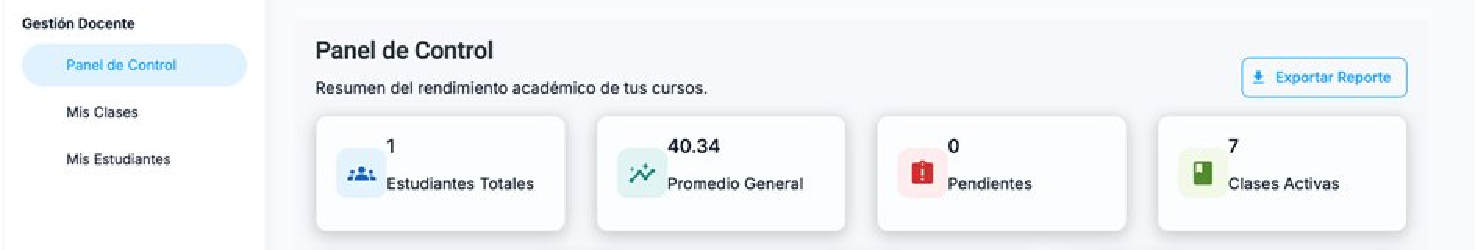
\includegraphics[width=0.92\textwidth,height=8cm,keepaspectratio]{figuras/ui_panel_control_docente.pdf}}\\\hline
Comentarios: & \multicolumn{3}{X|}{Los resultados deben poder ordenarse y compararse de alguna forma sencilla entre alumnos del mismo curso. Esta vista es el paso previo ideal para la generación de gráficas (CU-014) o exportación de datos (CU-015).}\\\hline
\end{tabularx}
\end{footnotesize}
\fuenteautor
\end{table}

\begin{table}[H]
\centering
\caption{Caso de uso ``Identificar brechas de aprendizaje''.}
\label{tab:cu_brechas}
\begin{footnotesize}
\renewcommand{\arraystretch}{1.25}
\begin{tabularx}{\textwidth}{|>{\bfseries}L{2.6cm}|X|>{\bfseries}L{2.4cm}|X|}
\hline
\rowcolor{tabhead}\multicolumn{4}{|c|}{\tabhead{Caso de uso ``Identificar brechas de aprendizaje''}}\\\hline
Código: & CU-016 & Actores: & Docente / Estudiante\\\hline
Objetivo: & \multicolumn{3}{X|}{Visualizar un análisis automático de los resultados categorizados por temas o competencias para identificar rápidamente las áreas de alto y bajo desempeño de los estudiantes (individual o grupal).}\\\hline
Resumen: & \multicolumn{3}{X|}{El sistema procesa el historial de evaluaciones, agrupa los aciertos y errores según la categoría temática de cada pregunta y presenta un resumen porcentual. Se utilizan colores semánticos e íconos para destacar visualmente el nivel de dominio en cada área.}\\\hline
Tipo: & \multicolumn{3}{X|}{Principal}\\\hline
Dependencias: & \multicolumn{3}{X|}{\textbf{Invoca a:} CU-017 (Sugerencias generadas por IA, que se alimentará de estos datos). \par \textbf{Depende de:} Resultados por evaluación y Categorización temática de preguntas en la base de datos.}\\\hline
Precondición: & \multicolumn{3}{X|}{El usuario (docente o estudiante) debe estar en la vista de análisis de rendimiento. Las evaluaciones realizadas deben contener preguntas previamente vinculadas a un tema o competencia curricular.}\\\hline
Postcondición: & \multicolumn{3}{X|}{El sistema procesa la información y renderiza en pantalla el análisis por categoría temática y el porcentaje de aciertos por área, destacando los extremos de desempeño.}\\\hline
[Importancia]: & \multicolumn{3}{X|}{Alta -- Permite una intervención pedagógica más precisa y la planificación de refuerzos o tutorías.}\\\hline
\rowcolor{tabhead2}\multicolumn{4}{|c|}{\textbf{Flujo normal de eventos}}\\\hline
\rowcolor{tabhead2}\multicolumn{2}{|>{\columncolor{tabhead2}}c|}{\textbf{Acción del actor}} & \multicolumn{2}{>{\columncolor{tabhead2}}c|}{\textbf{Respuesta del sistema}}\\\hline
\multicolumn{2}{|X|}{1.~El usuario (docente o estudiante) ingresa a la vista de análisis de áreas de desempeño (perfil individual o resumen del grupo).} & \multicolumn{2}{X|}{}\\\hline
\multicolumn{2}{|X|}{} & \multicolumn{2}{X|}{2.~El sistema recopila las respuestas del historial y lee la categoría temática de cada pregunta evaluada.}\\\hline
\multicolumn{2}{|X|}{} & \multicolumn{2}{X|}{3.~El sistema calcula el porcentaje de aciertos agrupado por cada categoría o competencia.}\\\hline
\multicolumn{2}{|X|}{} & \multicolumn{2}{X|}{4.~La aplicación renderiza una lista, tabla o gráfico con las áreas evaluadas.}\\\hline
\multicolumn{2}{|X|}{} & \multicolumn{2}{X|}{5.~El sistema aplica colores semánticos (ej. verde para áreas con alto porcentaje, rojo para bajo desempeño) e íconos distintivos.}\\\hline
\multicolumn{2}{|X|}{6.~El usuario visualiza la información y evalúa las áreas que requieren atención.} & \multicolumn{2}{X|}{}\\\hline
\multicolumn{2}{|X|}{} & \multicolumn{2}{X|}{7.~El sistema habilita la consulta de recomendaciones IA (CU-017) basándose en estos resultados.}\\\hline
\rowcolor{tabhead2}\multicolumn{4}{|c|}{\textbf{Flujo alterno}}\\\hline
\multicolumn{4}{|X|}{\textbf{2.a.\ Evaluaciones sin categorizar:} si las pruebas realizadas contienen preguntas que no fueron vinculadas a ningún tema, el sistema las agrupa bajo ``Categoría General'' o ``Sin clasificar'', o muestra una alerta al docente indicando que faltan metadatos para un análisis preciso.}\\\hline
\rowcolor{tabhead2}\multicolumn{4}{|c|}{\textbf{Diagrama de secuencia}}\\\hline
\multicolumn{4}{|c|}{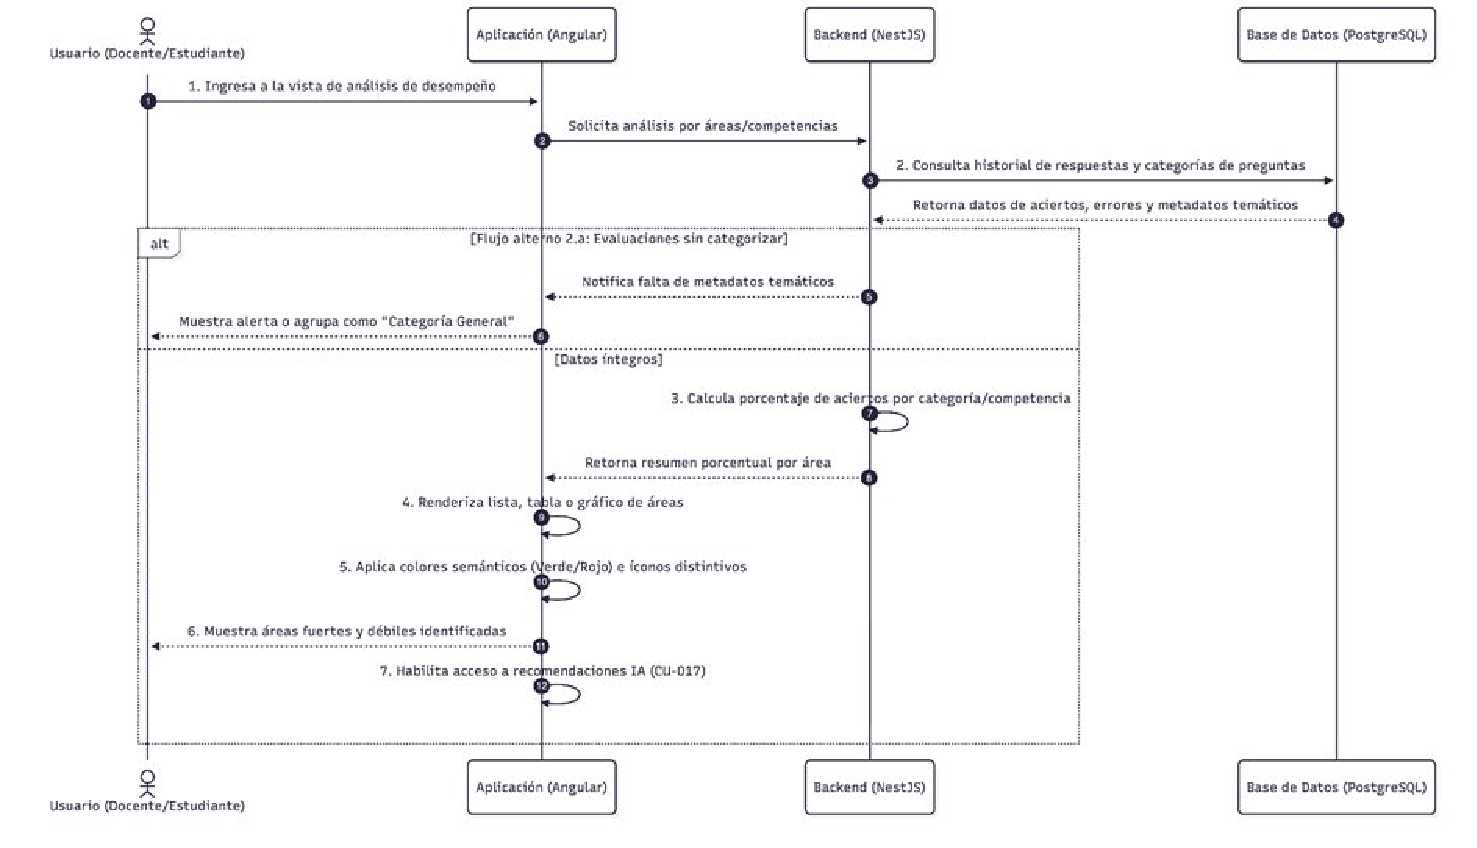
\includegraphics[width=0.92\textwidth,height=10cm,keepaspectratio]{figuras/seq_identificar_brechas.pdf}}\\\hline
\rowcolor{tabhead2}\multicolumn{4}{|c|}{\textbf{Interfaz de usuario}}\\\hline
\multicolumn{4}{|c|}{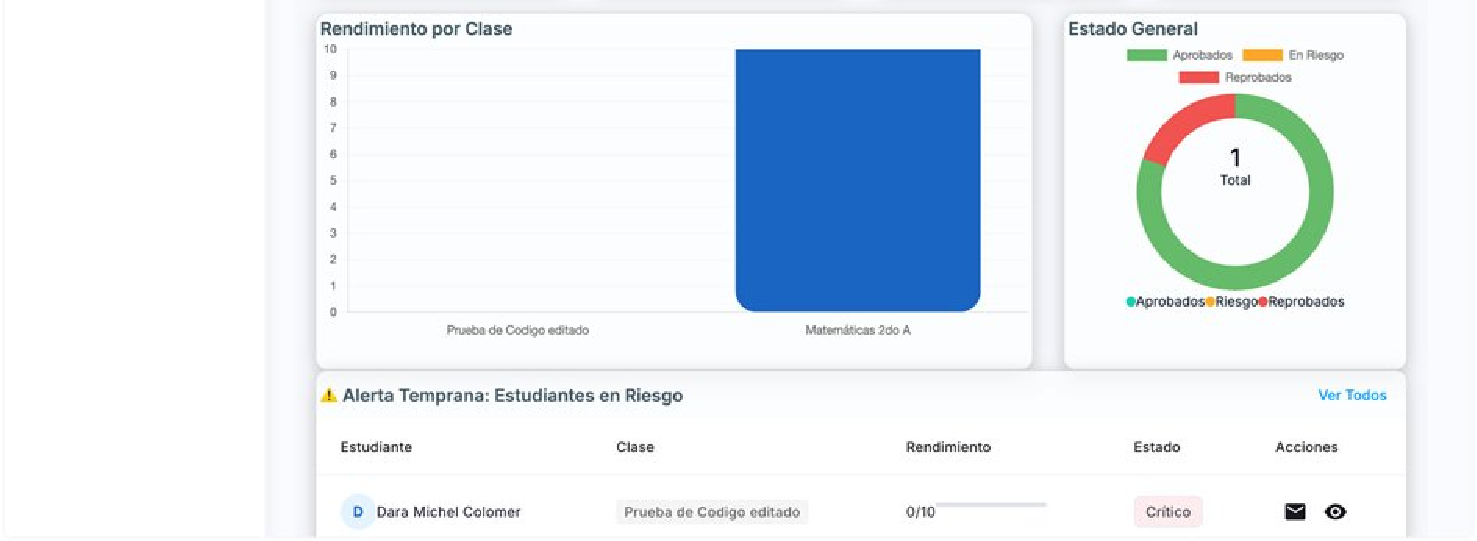
\includegraphics[width=0.92\textwidth,height=8cm,keepaspectratio]{figuras/ui_rendimiento_alertas.pdf}}\\\hline
Comentarios: & \multicolumn{3}{X|}{\textbf{Dependencia crítica:} para que este cálculo sea posible, el motor de evaluación debe categorizar cada pregunta por tema en la base de datos al momento de crearla (CU-010).}\\\hline
\end{tabularx}
\end{footnotesize}
\fuenteautor
\end{table}

\begin{table}[H]
\centering
\caption{Caso de uso ``Recibir consejos IA''.}
\label{tab:cu_consejos}
\begin{footnotesize}
\renewcommand{\arraystretch}{1.25}
\begin{tabularx}{\textwidth}{|>{\bfseries}L{2.6cm}|X|>{\bfseries}L{2.4cm}|X|}
\hline
\rowcolor{tabhead}\multicolumn{4}{|c|}{\tabhead{Caso de uso ``Recibir consejos IA''}}\\\hline
Código: & CU-017 & Actores: & Docente / Estudiante\\\hline
Objetivo: & \multicolumn{3}{X|}{Recibir sugerencias automáticas basadas en el análisis de los patrones de error y evaluaciones anteriores para saber exactamente qué temas y competencias reforzar.}\\\hline
Resumen: & \multicolumn{3}{X|}{El sistema utiliza un modelo de IA para analizar el historial de resultados del estudiante, detectar áreas de bajo rendimiento y generar recomendaciones textuales breves y prácticas tanto para el autoestudio del alumno como para la planificación del docente.}\\\hline
Tipo: & \multicolumn{3}{X|}{Principal}\\\hline
Dependencias: & \multicolumn{3}{X|}{\textbf{Invoca a:} ninguno directamente. \par \textbf{Depende de:} Análisis de resultados (CU-016) y Modelo de recomendación IA.}\\\hline
Precondición: & \multicolumn{3}{X|}{El estudiante debe contar con un historial de evaluaciones completadas y procesadas por el módulo de análisis de resultados (CU-016). El motor de IA debe tener acceso a los patrones de error y competencias evaluadas.}\\\hline
Postcondición: & \multicolumn{3}{X|}{El sistema procesa la información y devuelve sugerencias textuales que cumplen con tener un formato breve, claro y práctico. Estas sugerencias se desglosan por estudiante y por competencia.}\\\hline
[Importancia]: & \multicolumn{3}{X|}{Alta -- Fomenta el aprendizaje adaptativo y personalizado.}\\\hline
\rowcolor{tabhead2}\multicolumn{4}{|c|}{\textbf{Flujo normal de eventos}}\\\hline
\rowcolor{tabhead2}\multicolumn{2}{|>{\columncolor{tabhead2}}c|}{\textbf{Acción del actor}} & \multicolumn{2}{>{\columncolor{tabhead2}}c|}{\textbf{Respuesta del sistema}}\\\hline
\multicolumn{2}{|X|}{1.~El usuario (estudiante o docente) ingresa al panel de retroalimentación o resultados del alumno.} & \multicolumn{2}{X|}{}\\\hline
\multicolumn{2}{|X|}{} & \multicolumn{2}{X|}{2.~El sistema analiza automáticamente los resultados anteriores del estudiante para detectar competencias con bajo rendimiento.}\\\hline
\multicolumn{2}{|X|}{} & \multicolumn{2}{X|}{3.~El motor de IA procesa los patrones de error identificados en la base de datos.}\\\hline
\multicolumn{2}{|X|}{} & \multicolumn{2}{X|}{4.~El sistema genera sugerencias personalizadas por cada estudiante y por competencia específica.}\\\hline
\multicolumn{2}{|X|}{} & \multicolumn{2}{X|}{5.~La aplicación presenta las recomendaciones en pantalla mediante un formato de texto breve, claro y práctico.}\\\hline
\rowcolor{tabhead2}\multicolumn{4}{|c|}{\textbf{Flujo alterno}}\\\hline
\multicolumn{4}{|X|}{\textbf{2.a.\ Historial insuficiente:} si el estudiante no tiene suficientes evaluaciones o errores para analizar, el sistema mostrará un mensaje indicando que se requiere más información de pruebas o que el estudiante mantiene un rendimiento óptimo general. \par \textbf{3.a.\ Error del servicio de IA:} si la comunicación con el modelo de recomendación falla, el sistema oculta temporalmente la sección de sugerencias y muestra un mensaje amigable indicando que las recomendaciones no están disponibles en ese momento.}\\\hline
\rowcolor{tabhead2}\multicolumn{4}{|c|}{\textbf{Diagrama de secuencia}}\\\hline
\multicolumn{4}{|c|}{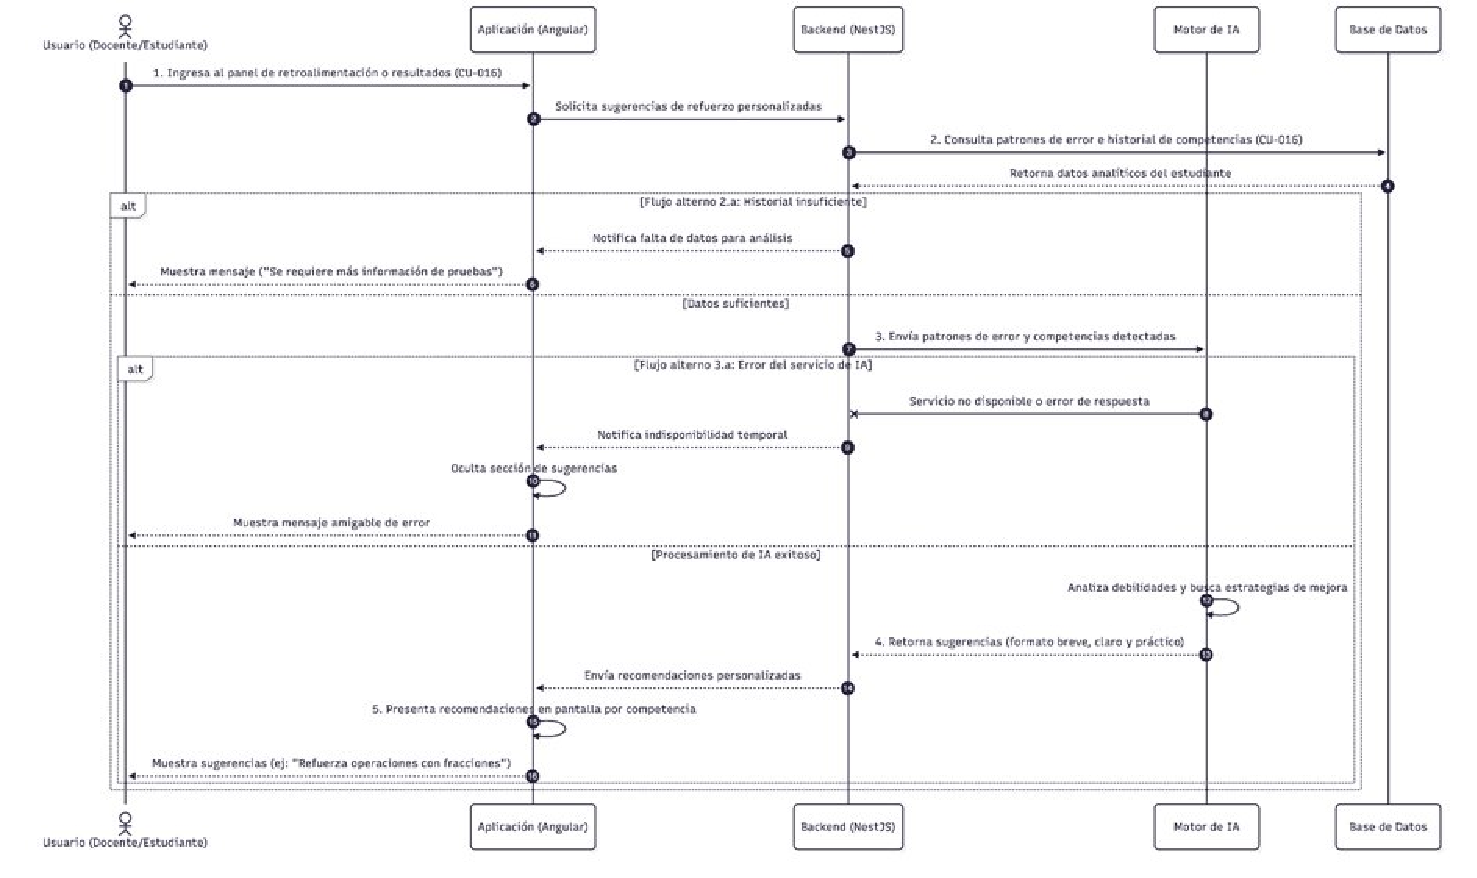
\includegraphics[width=0.92\textwidth,height=10cm,keepaspectratio]{figuras/seq_recibir_consejos_ia.pdf}}\\\hline
\rowcolor{tabhead2}\multicolumn{4}{|c|}{\textbf{Interfaz de usuario}}\\\hline
\multicolumn{4}{|c|}{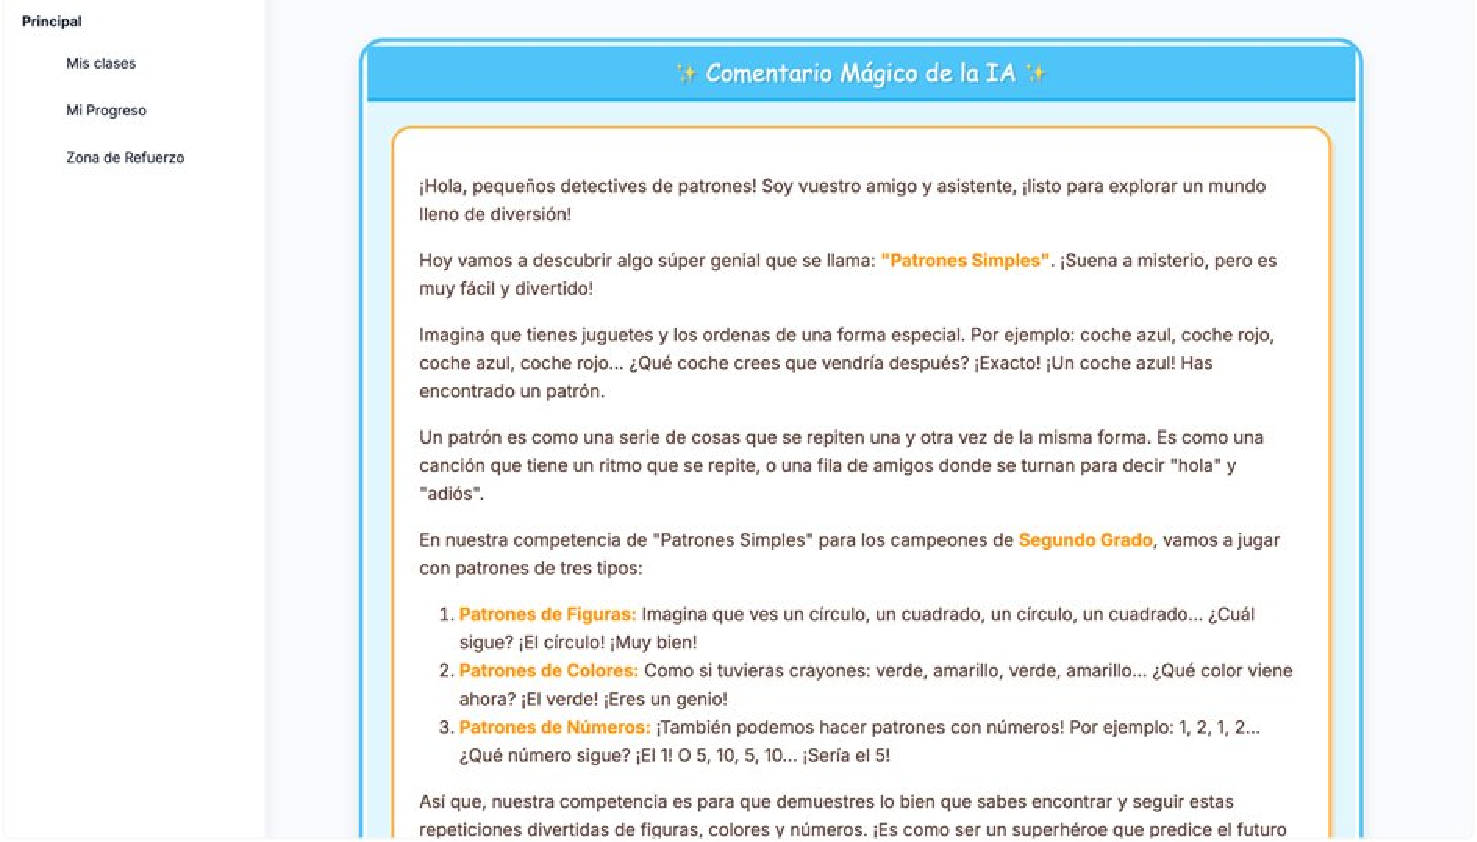
\includegraphics[width=0.92\textwidth,height=8cm,keepaspectratio]{figuras/ui_comentario_magico_ia.pdf}}\\\hline
Comentarios: & \multicolumn{3}{X|}{Las sugerencias pueden incluir frases directas como: ``Refuerza operaciones con fracciones'' o ``Revisa conceptos de geometría básica''. Estas recomendaciones deben ser visibles tanto en el panel del estudiante (para su autoestudio) como en la vista de resultados del docente (para su planificación).}\\\hline
\end{tabularx}
\end{footnotesize}
\fuenteautor
\end{table}

\begin{table}[H]
\centering
\caption{Caso de uso ``Aplicar gamificación''.}
\label{tab:cu_gamificacion}
\begin{footnotesize}
\renewcommand{\arraystretch}{1.25}
\begin{tabularx}{\textwidth}{|>{\bfseries}L{2.6cm}|X|>{\bfseries}L{2.4cm}|X|}
\hline
\rowcolor{tabhead}\multicolumn{4}{|c|}{\tabhead{Caso de uso ``Aplicar gamificación''}}\\\hline
Código: & CU-021 & Actores: & Estudiante\\\hline
Objetivo: & \multicolumn{3}{X|}{Otorgar insignias visuales y puntos al estudiante tras completar evaluaciones exitosamente o alcanzar metas de aprendizaje, para mantener un alto nivel de motivación.}\\\hline
Resumen: & \multicolumn{3}{X|}{El sistema evalúa el rendimiento y el progreso del alumno al finalizar una prueba. Si cumple ciertos criterios predefinidos (ej. nota perfecta, racha de tres pruebas seguidas), desbloquea un logro en su perfil, notificándole con una animación celebratoria.}\\\hline
Tipo: & \multicolumn{3}{X|}{Principal}\\\hline
Dependencias: & \multicolumn{3}{X|}{\textbf{Invoca a:} actualización del perfil del estudiante. \par \textbf{Depende de:} CU-005 (Presentación de resultados) y del motor de reglas de gamificación en el \textit{backend}.}\\\hline
Precondición: & \multicolumn{3}{X|}{El estudiante debe haber finalizado satisfactoriamente una evaluación (CU-004/CU-005). Deben existir insignias previamente configuradas en la base de datos con sus respectivas condiciones de desbloqueo.}\\\hline
Postcondición: & \multicolumn{3}{X|}{El sistema registra el nuevo logro obtenido vinculándolo al ID del estudiante en la base de datos (PostgreSQL) y este pasa a estar visible de forma permanente en su ``vitrina de logros'' virtual.}\\\hline
[Importancia]: & \multicolumn{3}{X|}{Alta -- Esencial para retener la atención y fomentar el esfuerzo continuo en niños de primaria.}\\\hline
\rowcolor{tabhead2}\multicolumn{4}{|c|}{\textbf{Flujo normal de eventos}}\\\hline
\rowcolor{tabhead2}\multicolumn{2}{|>{\columncolor{tabhead2}}c|}{\textbf{Acción del actor}} & \multicolumn{2}{>{\columncolor{tabhead2}}c|}{\textbf{Respuesta del sistema}}\\\hline
\multicolumn{2}{|X|}{1.~El estudiante finaliza su evaluación y llega a la pantalla de resultados (CU-005).} & \multicolumn{2}{X|}{}\\\hline
\multicolumn{2}{|X|}{} & \multicolumn{2}{X|}{2.~El sistema recibe los resultados y los envía al motor de validación de logros.}\\\hline
\multicolumn{2}{|X|}{} & \multicolumn{2}{X|}{3.~El sistema compara el puntaje y el historial del alumno contra las reglas de las insignias bloqueadas.}\\\hline
\multicolumn{2}{|X|}{} & \multicolumn{2}{X|}{4.~El sistema determina que el estudiante ha cumplido la condición para un nuevo logro (ej. ``Genio Matemático'').}\\\hline
\multicolumn{2}{|X|}{} & \multicolumn{2}{X|}{5.~El sistema registra el logro como ``desbloqueado'' en la base de datos para ese usuario.}\\\hline
\multicolumn{2}{|X|}{} & \multicolumn{2}{X|}{6.~La aplicación superpone una animación festiva y llamativa en pantalla anunciando la nueva medalla o insignia.}\\\hline
\multicolumn{2}{|X|}{7.~El estudiante hace clic en ``Continuar'' o ``Ver mis logros''.} & \multicolumn{2}{X|}{}\\\hline
\multicolumn{2}{|X|}{} & \multicolumn{2}{X|}{8.~El sistema redirige al estudiante a su panel principal o a su vitrina de insignias, actualizando su contador de recompensas.}\\\hline
\rowcolor{tabhead2}\multicolumn{4}{|c|}{\textbf{Flujo alterno}}\\\hline
\multicolumn{4}{|X|}{\textbf{4.a.} Si el estudiante no cumple con ninguna condición nueva tras la evaluación, el sistema simplemente omite la animación de desbloqueo y muestra únicamente la retroalimentación normal de la prueba. \par \textbf{6.a.} Si ocurre un fallo de conexión al intentar guardar el logro, el sistema lo almacena en caché temporalmente y reintenta la sincronización en segundo plano sin interrumpir la experiencia del alumno.}\\\hline
\rowcolor{tabhead2}\multicolumn{4}{|c|}{\textbf{Diagrama de secuencia}}\\\hline
\multicolumn{4}{|c|}{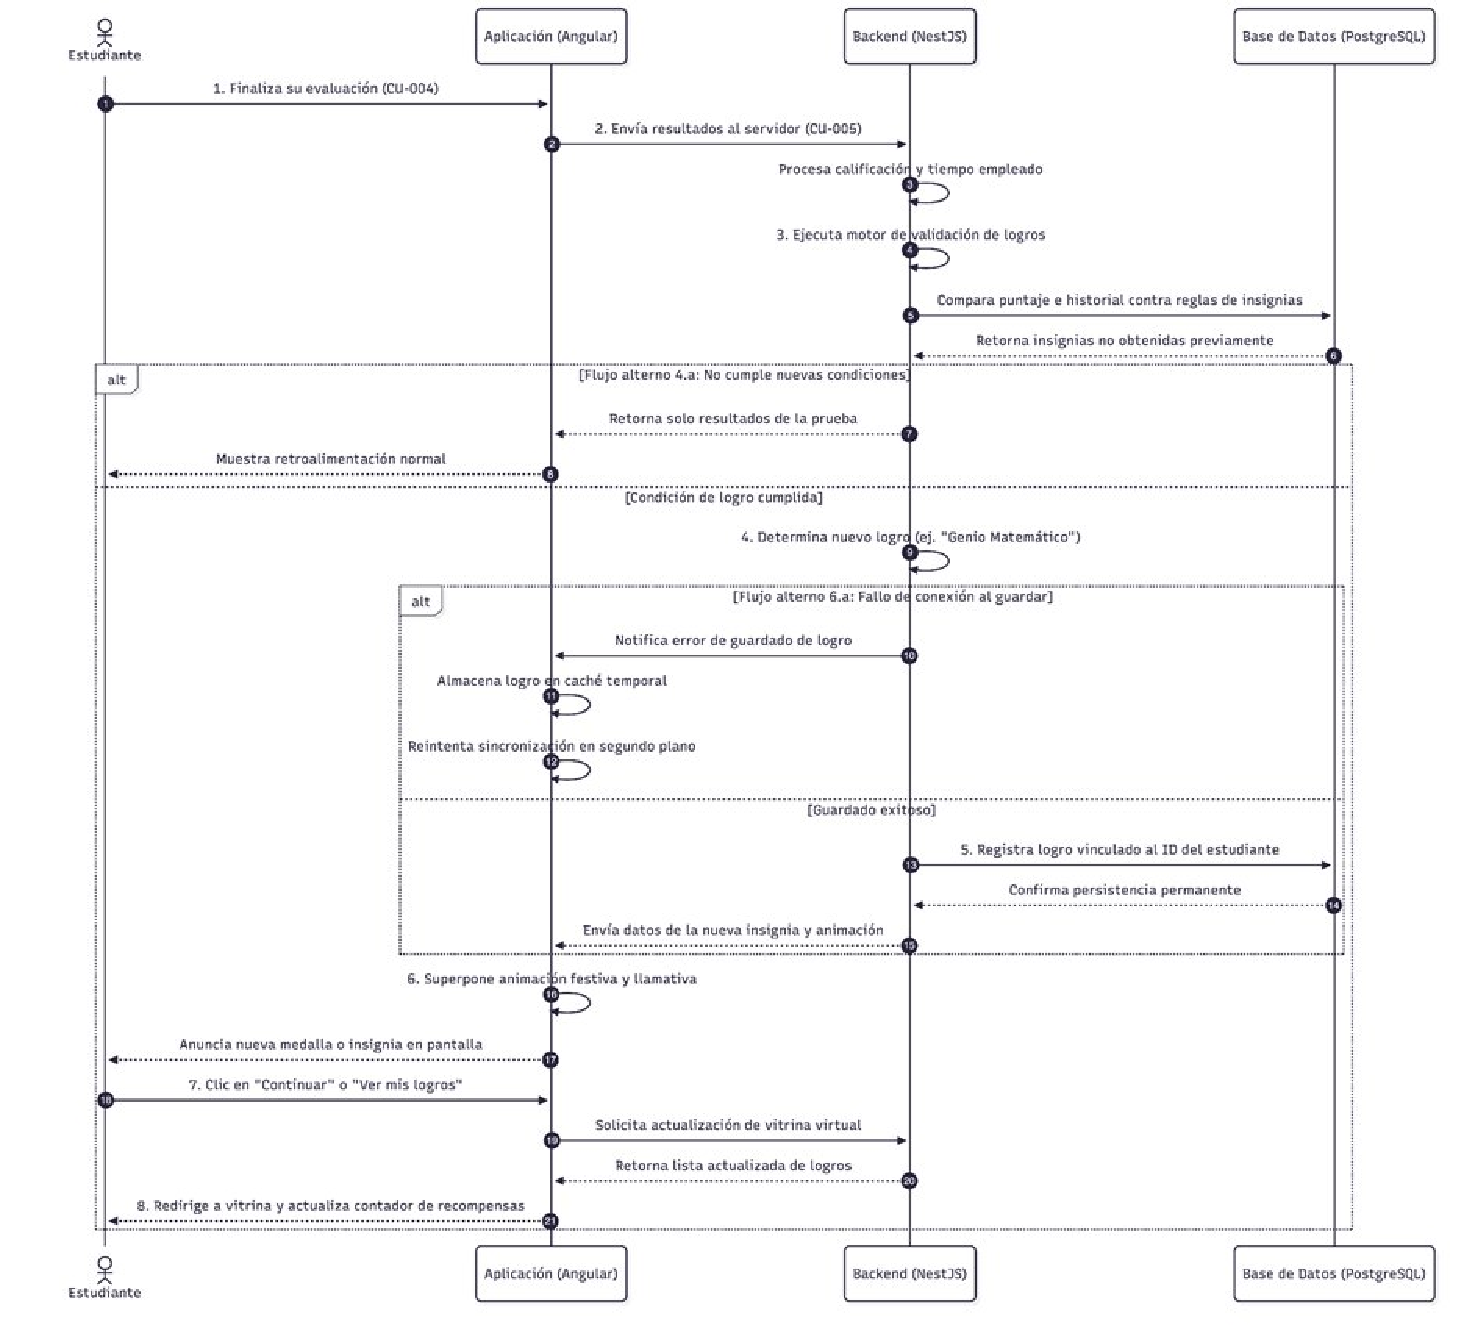
\includegraphics[width=0.92\textwidth,height=10cm,keepaspectratio]{figuras/seq_aplicar_gamificacion.pdf}}\\\hline
\rowcolor{tabhead2}\multicolumn{4}{|c|}{\textbf{Interfaz de usuario}}\\\hline
\multicolumn{4}{|c|}{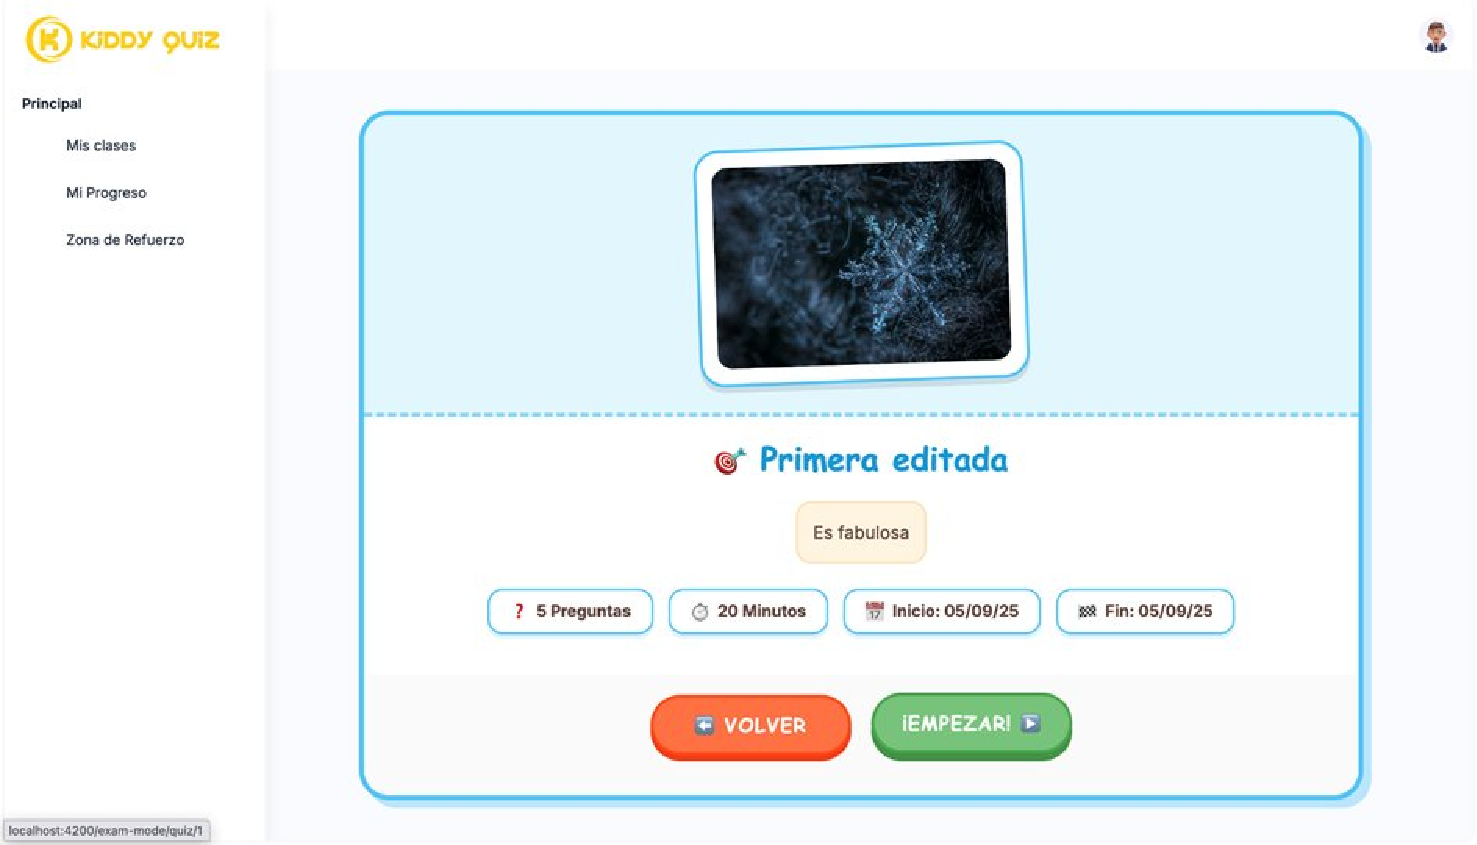
\includegraphics[width=0.92\textwidth,height=8cm,keepaspectratio]{figuras/ui_pre_evaluacion.pdf}}\\\hline
Comentarios: & \multicolumn{3}{X|}{Las insignias deben tener un diseño muy visual, tipo ``cartoon'' o videojuego, aprovechando Angular para las animaciones CSS. Se recomienda incluir una barra de progreso que le indique al niño cuánto le falta para su próxima recompensa.}\\\hline
\end{tabularx}
\end{footnotesize}
\fuenteautor
\end{table}

\begin{table}[H]
\centering
\caption{Caso de uso ``Ingresar a clase''.}
\label{tab:cu_ingresar}
\begin{footnotesize}
\renewcommand{\arraystretch}{1.25}
\begin{tabularx}{\textwidth}{|>{\bfseries}L{2.6cm}|X|>{\bfseries}L{2.4cm}|X|}
\hline
\rowcolor{tabhead}\multicolumn{4}{|c|}{\tabhead{Caso de uso ``Ingresar a clase''}}\\\hline
Código: & CU-027 & Actores: & Estudiante\\\hline
Objetivo: & \multicolumn{3}{X|}{Permitir al estudiante vincularse a una clase o grupo específico administrado por su docente mediante la introducción de un código único.}\\\hline
Resumen: & \multicolumn{3}{X|}{El estudiante ingresa un código alfanumérico corto proporcionado por su profesor. El sistema valida este código y, de ser correcto, inscribe al alumno en el curso correspondiente, dándole acceso inmediato a sus evaluaciones.}\\\hline
Tipo: & \multicolumn{3}{X|}{Principal / Vinculación}\\\hline
Dependencias: & \multicolumn{3}{X|}{\textbf{Invoca a:} afecta directamente al CU-003 (Visualización de evaluaciones disponibles), ya que habilitará nuevo contenido. \par \textbf{Depende de:} CU-001 (Inicio de sesión) y de que el docente haya generado y compartido el código previamente.}\\\hline
Precondición: & \multicolumn{3}{X|}{El estudiante debe haber iniciado sesión exitosamente en su panel. El docente debe haber creado una clase en el sistema y el código de vinculación debe estar activo.}\\\hline
Postcondición: & \multicolumn{3}{X|}{El estudiante queda asociado a la clase y al docente en la base de datos (PostgreSQL). El sistema actualiza el panel del estudiante, otorgándole acceso a las evaluaciones que estén habilitadas para ese curso específico.}\\\hline
[Importancia]: & \multicolumn{3}{X|}{Muy alta -- Es el mecanismo principal para estructurar los grupos de alumnos y conectar docentes con estudiantes.}\\\hline
\rowcolor{tabhead2}\multicolumn{4}{|c|}{\textbf{Flujo normal de eventos}}\\\hline
\rowcolor{tabhead2}\multicolumn{2}{|>{\columncolor{tabhead2}}c|}{\textbf{Acción del actor}} & \multicolumn{2}{>{\columncolor{tabhead2}}c|}{\textbf{Respuesta del sistema}}\\\hline
\multicolumn{2}{|X|}{1.~El estudiante selecciona la opción ``Unirse a una clase'' en su panel principal.} & \multicolumn{2}{X|}{}\\\hline
\multicolumn{2}{|X|}{} & \multicolumn{2}{X|}{2.~El sistema despliega un \textit{modal} o pantalla con un campo de texto simple y un botón de confirmación.}\\\hline
\multicolumn{2}{|X|}{3.~El estudiante ingresa el código único proporcionado por el docente y hace clic en ``Unirse''.} & \multicolumn{2}{X|}{}\\\hline
\multicolumn{2}{|X|}{} & \multicolumn{2}{X|}{4.~El sistema recibe el código y lo consulta en la base de datos de cursos.}\\\hline
\multicolumn{2}{|X|}{} & \multicolumn{2}{X|}{5.~El sistema verifica que el código es válido, corresponde a una clase activa y que el alumno no está previamente inscrito en ella.}\\\hline
\multicolumn{2}{|X|}{} & \multicolumn{2}{X|}{6.~El sistema crea la asociación (llaves foráneas) entre el ID del estudiante y el ID de la clase/docente.}\\\hline
\multicolumn{2}{|X|}{} & \multicolumn{2}{X|}{7.~La aplicación muestra una animación festiva y un mensaje de éxito indicando el nombre de la clase a la que se unió (ej. ``¡Bienvenido a 4to Grado de Matemáticas!'').}\\\hline
\multicolumn{2}{|X|}{8.~El estudiante hace clic en ``Ir a mis pruebas''.} & \multicolumn{2}{X|}{}\\\hline
\multicolumn{2}{|X|}{} & \multicolumn{2}{X|}{9.~El sistema redirige al panel principal (CU-003), recargando la vista para mostrar las tarjetas de evaluaciones de su nueva clase.}\\\hline
\rowcolor{tabhead2}\multicolumn{4}{|c|}{\textbf{Flujo alterno}}\\\hline
\multicolumn{4}{|X|}{\textbf{5.a.\ Código inválido o inactivo:} si el código no existe o el docente lo desactivó, el sistema muestra un mensaje amigable (ej. ``¡Ups! Ese código no funciona. Revisa si lo copiaste bien o pregúntale a tu profe'') y limpia el campo para reintentar. \par \textbf{5.b.\ Alumno ya inscrito:} si el sistema detecta que el estudiante ya pertenece a ese grupo, muestra una alerta indicando ``¡Ya eres parte de esta clase!'' y cancela el proceso de vinculación redundante.}\\\hline
\rowcolor{tabhead2}\multicolumn{4}{|c|}{\textbf{Diagrama de secuencia}}\\\hline
\multicolumn{4}{|c|}{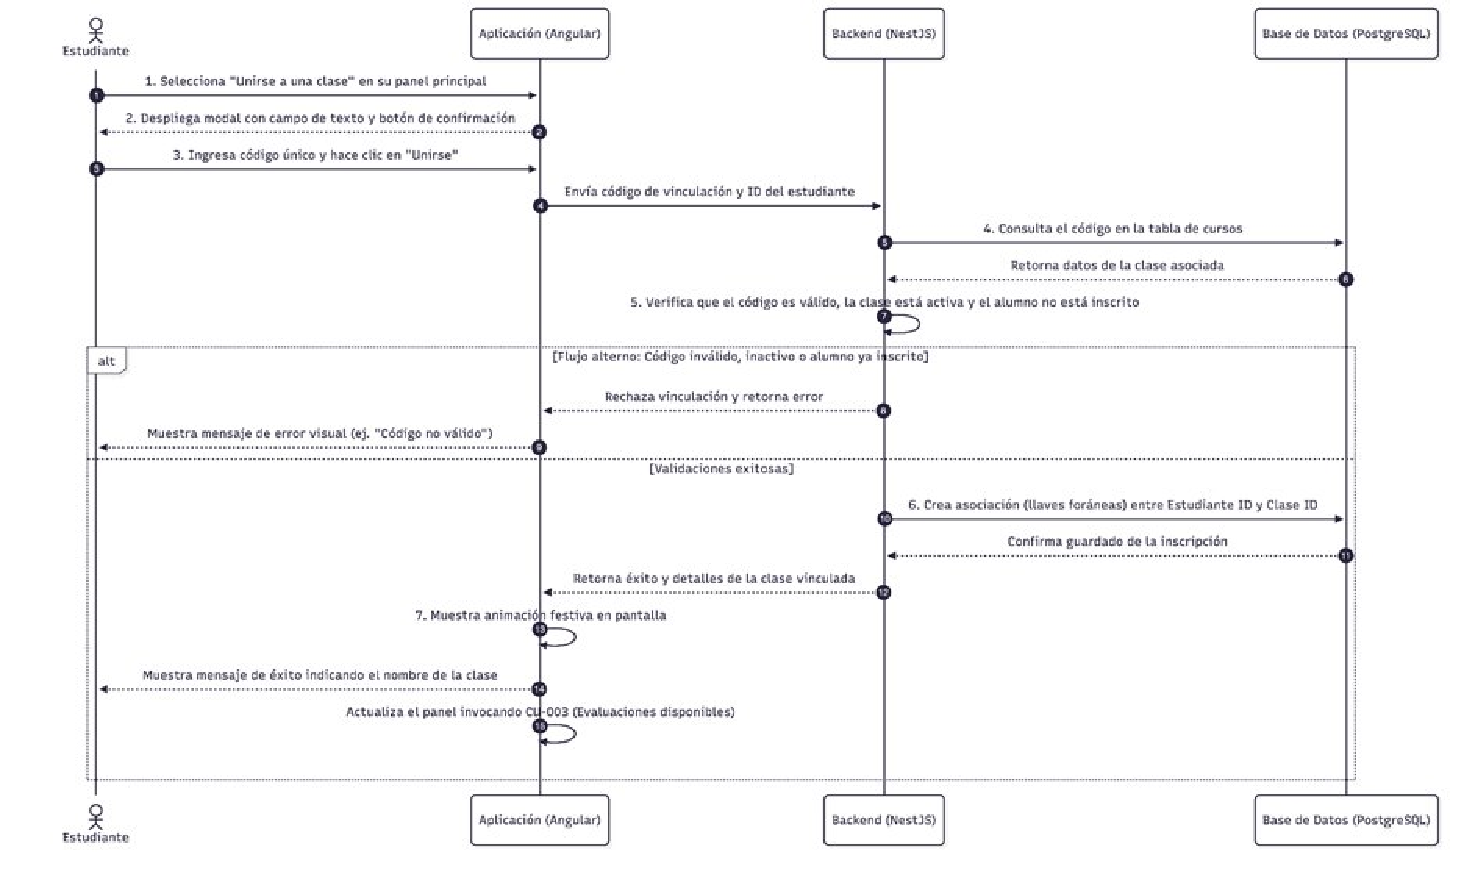
\includegraphics[width=0.92\textwidth,height=10cm,keepaspectratio]{figuras/seq_ingresar_clase.pdf}}\\\hline
\rowcolor{tabhead2}\multicolumn{4}{|c|}{\textbf{Interfaz de usuario}}\\\hline
\multicolumn{4}{|c|}{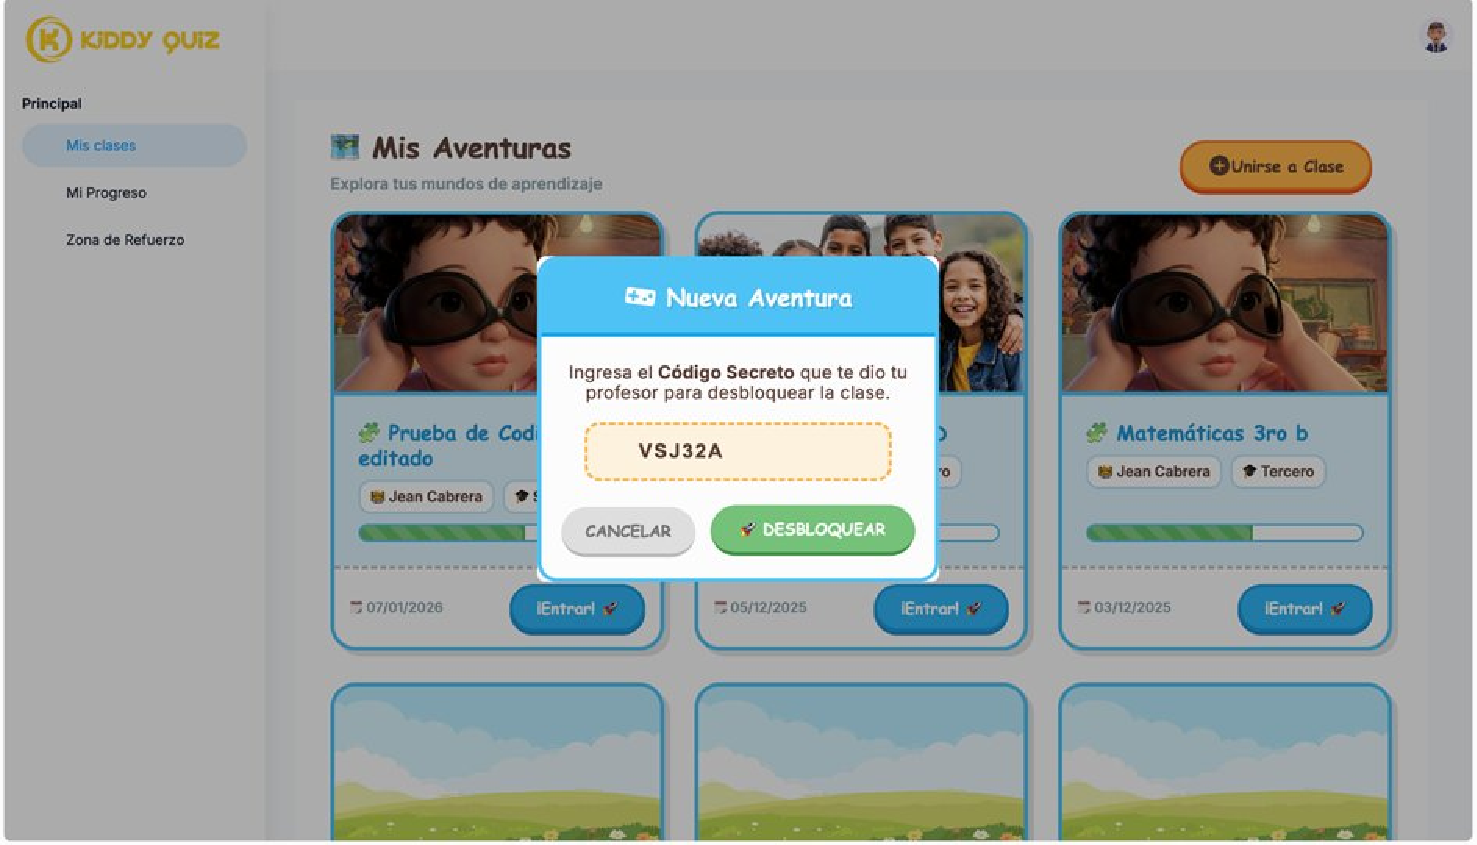
\includegraphics[width=0.92\textwidth,height=8cm,keepaspectratio]{figuras/ui_ingresar_codigo.pdf}}\\\hline
Comentarios: & \multicolumn{3}{X|}{El campo para ingresar el código debe ser grande, con tipografía clara y estar configurado en Angular para no distinguir entre mayúsculas y minúsculas (\textit{case-insensitive}), evitando así frustraciones comunes en niños de educación básica.}\\\hline
\end{tabularx}
\end{footnotesize}
\fuenteautor
\end{table}

\begin{table}[H]
\centering
\caption{Caso de uso ``Ver mapa de competencias''.}
\label{tab:cu_mapa}
\begin{footnotesize}
\renewcommand{\arraystretch}{1.25}
\begin{tabularx}{\textwidth}{|>{\bfseries}L{2.6cm}|X|>{\bfseries}L{2.4cm}|X|}
\hline
\rowcolor{tabhead}\multicolumn{4}{|c|}{\tabhead{Caso de uso ``Ver mapa de competencias''}}\\\hline
Código: & CU-026 & Actores: & Docente / Estudiante\\\hline
Objetivo: & \multicolumn{3}{X|}{Mostrar un mapa visual por estudiante que refleje qué competencias curriculares han sido evaluadas y cuáles ha logrado alcanzar.}\\\hline
Resumen: & \multicolumn{3}{X|}{El sistema despliega una lista de competencias por módulo y nivel, indicando el estado de cada una (lograda, en proceso, no iniciada) mediante una visualización gráfica de cuadros, íconos y colores. Se habilita la opción de exportar este mapa en formato PDF o Excel.}\\\hline
Tipo: & \multicolumn{3}{X|}{Principal}\\\hline
Dependencias: & \multicolumn{3}{X|}{\textbf{Invoca a:} CU-015 (Exportación de resultados) para la generación del PDF. \par \textbf{Depende de:} Motor de resultados y Base de datos de competencias curriculares.}\\\hline
Precondición: & \multicolumn{3}{X|}{El estudiante debe haber completado evaluaciones que tengan competencias curriculares vinculadas. El usuario debe estar autenticado para acceder a su perfil o al de sus alumnos.}\\\hline
Postcondición: & \multicolumn{3}{X|}{El sistema despliega una lista de competencias por módulo y nivel, indicando el estado de cada una mediante una visualización gráfica. Se habilita la opción de exportar este mapa en formato PDF o Excel.}\\\hline
[Importancia]: & \multicolumn{3}{X|}{Alta -- Refuerza el enfoque por competencias y la toma de decisiones pedagógicas.}\\\hline
\rowcolor{tabhead2}\multicolumn{4}{|c|}{\textbf{Flujo normal de eventos}}\\\hline
\rowcolor{tabhead2}\multicolumn{2}{|>{\columncolor{tabhead2}}c|}{\textbf{Acción del actor}} & \multicolumn{2}{>{\columncolor{tabhead2}}c|}{\textbf{Respuesta del sistema}}\\\hline
\multicolumn{2}{|X|}{1.~El usuario (docente o estudiante) consulta el progreso académico en la plataforma.} & \multicolumn{2}{X|}{}\\\hline
\multicolumn{2}{|X|}{} & \multicolumn{2}{X|}{2.~El sistema recupera el historial de evaluaciones del alumno y consulta la base de datos de competencias curriculares.}\\\hline
\multicolumn{2}{|X|}{} & \multicolumn{2}{X|}{3.~El sistema calcula el estado actual de cada competencia evaluada.}\\\hline
\multicolumn{2}{|X|}{} & \multicolumn{2}{X|}{4.~El sistema despliega una lista de competencias organizadas por módulo y nivel.}\\\hline
\multicolumn{2}{|X|}{} & \multicolumn{2}{X|}{5.~La aplicación indica visualmente si la competencia está lograda, en proceso o no iniciada mediante cuadros, íconos y colores.}\\\hline
\multicolumn{2}{|X|}{6.~El usuario selecciona la opción para exportar el mapa de competencias.} & \multicolumn{2}{X|}{}\\\hline
\multicolumn{2}{|X|}{} & \multicolumn{2}{X|}{7.~El sistema invoca el módulo de exportación (CU-015) y genera el archivo en formato PDF o Excel.}\\\hline
\rowcolor{tabhead2}\multicolumn{4}{|c|}{\textbf{Flujo alterno}}\\\hline
\multicolumn{4}{|X|}{\textbf{2.a.\ Sin datos previos:} si el estudiante no ha realizado ninguna evaluación con competencias vinculadas, el mapa mostrará todas las áreas en estado ``no iniciada'' y sugerirá realizar una prueba diagnóstica.}\\\hline
\rowcolor{tabhead2}\multicolumn{4}{|c|}{\textbf{Diagrama de secuencia}}\\\hline
\multicolumn{4}{|c|}{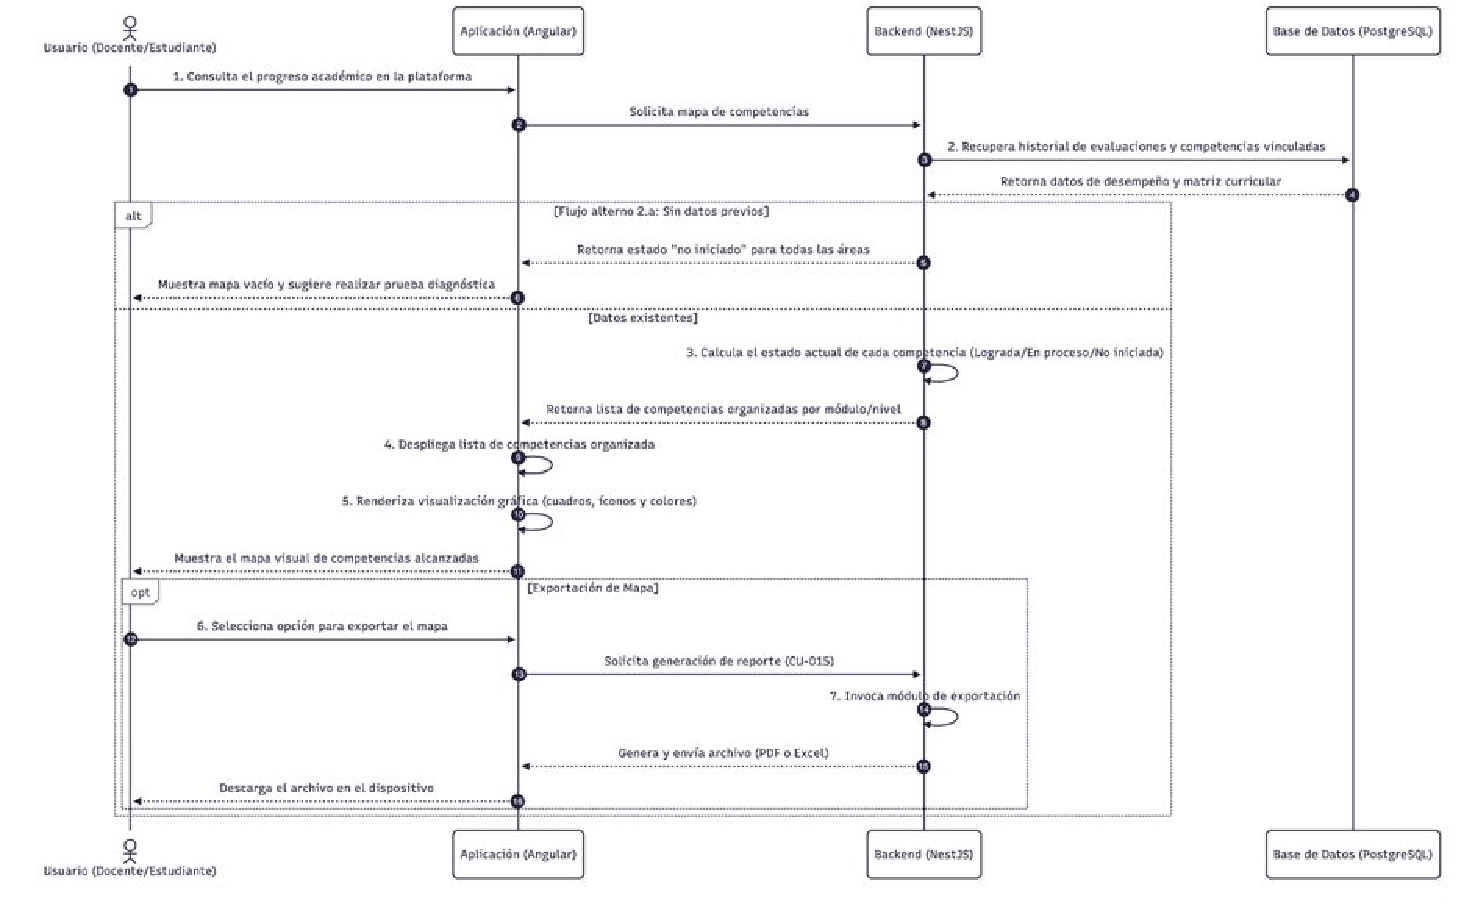
\includegraphics[width=0.92\textwidth,height=10cm,keepaspectratio]{figuras/seq_mapa_competencias.pdf}}\\\hline
\rowcolor{tabhead2}\multicolumn{4}{|c|}{\textbf{Interfaz de usuario}}\\\hline
\multicolumn{4}{|c|}{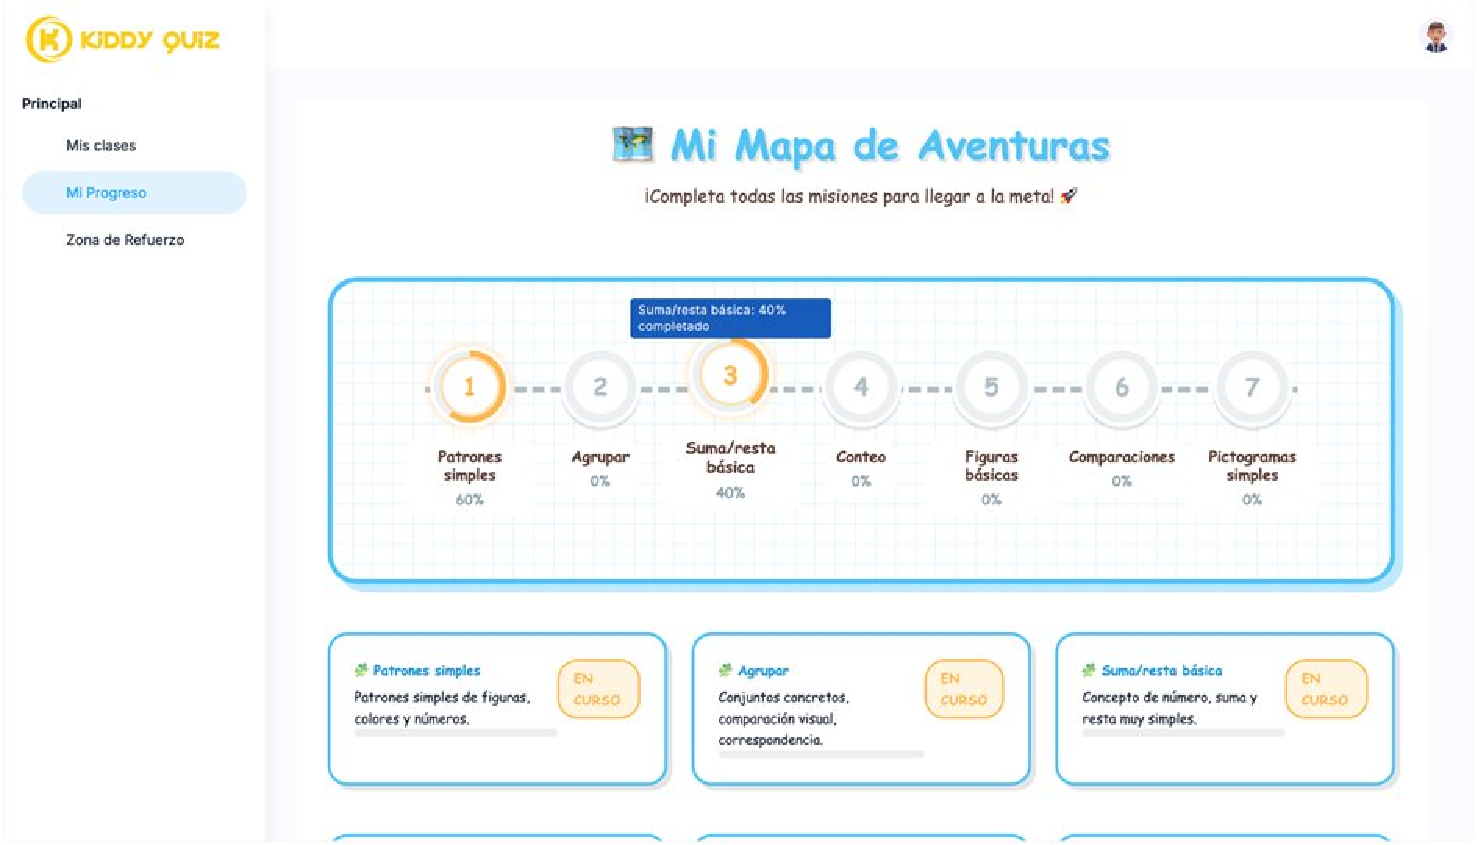
\includegraphics[width=0.92\textwidth,height=8cm,keepaspectratio]{figuras/ui_mapa_aventuras.pdf}}\\\hline
Comentarios: & \multicolumn{3}{X|}{El mapa debe actualizarse en tiempo real tras cada evaluación. Puede usarse como excelente herramienta de comunicación directa con padres o representantes.}\\\hline
\end{tabularx}
\end{footnotesize}
\fuenteautor
\end{table}
